\chapter{Introduction}
Formal models such as grammars and automata have a long history in theoretical computer science, where they play a foundational role in areas such as computability, decidability, and computational complexity. In practice, they are irreplaceable in compiler design, where they are used for lexical analysis, syntax parsing, and semantic interpretation. However, their applicability extends far beyond the domain of computer science. These models have also been found to be relevant in fields such as biology, linguistics, visual arts, and music.

As the title of this thesis already suggests, the work will focus on music and music composition. Music composition was, for a long time, viewed as a domain for humans and their creativity. With the rise of formal modeling techniques, this trend changed significantly. Music could be compared to language. It exhibits structural dependencies, repetitions, variations, and other compositional aspects that make music open to formal models such as grammars, automata, and others. They can be used to describe musical syntax, generate melodies, and even model complex harmonic progressions. Researchers also developed many musically meaningful transformation techniques that modify notes and chords in musically meaningful ways.

Formal models combined with music are a strange combination. Some can question how it is possible to find real-life applications. They can not replicate human emotion, which is often a thing that makes music expressive and engaging. Furthermore, one might ask whether this approach can compete with modern solutions, such as neural networks, which start to dominate generative music. The structured and interpretable nature of formal models makes them a great complementary tool in music generation. There are also areas where performance constraints still play a role, which makes formal approaches more suitable than neural networks. In this work, we demonstrate their potential by presenting several areas where they can be effectively applied to produce explainable and reusable music.

In the modern era, computer scientists working in the field of formal models face the issue that the mathematical development of those models surpassed their application. Rather than extending this gap, this work tries to close it with novel approach to instrument synchronization in polyphonic music generation based on formal grammar systems. This direction was taken in response to limitations observed in existing grammar-based music generation approaches. These limitations arise from challenges on both the technical and artistic sides. Although existing formal models are often used correctly from a computational standpoint, they tend to lack the flexibility required for broader musical applications. As a result, they are typically restricted to generating simple melodies, short passages, or isolated musical ideas, rather than producing coherent, expressive, and extended polyphonic compositions.

Before addressing these questions and presenting a solution, the reader must first be familiar with the fundamentals of formal languages and models, which are introduced in Chapter~\ref{chap1}. This chapter gives a small overview of what models are used in musicology and how they are categorized with respect to their generative power.

Chapter~\ref{chap2} is a key to understanding how the model works and how grammatical rules are designed. After this chapter, a reader should be able to create his own rules for the components of the grammar system and generate meaningful melodies or harmonies. It explains that music is still an art and there is no such thing as correct music. The output of the system may appeal to somebody and not to others. Later in this chapter, we provide an explanation for the selection of the model and how it relates to music and its structural properties.

Chapter~\ref{chap3} reviews related work in grammar-based music generation and outlines how this thesis contributes to and differentiates itself from existing approaches.

The core contribution of this thesis is presented in Chapter~\ref{chap4} and Chapter~\ref{chap5}. In Chapter~\ref{chap4}, we introduce the design of a rule-synchronized grammar system that incorporates components in the form of scattered context grammars. The chapter provides a detailed explanation of how melody and harmony can be encoded into grammatical rules and how compositional structure is represented through them, and it includes illustrative examples based on both jazz and classical music. Furthermore, a generation algorithm is proposed and described, serving as the basis for music production within this framework.

Chapter~\ref{chap5} focuses on the implementation of this system. It describes the software architecture, input format, and system behavior. The implementation is evaluated and compared with several existing and popular approaches, both from academic literature and open-source repositories such as GitHub.

\chapter{Formal languages and grammars}
\label{chap1}
From the literature, we already know that formal models are applied in many scientific fields. The applications we can find are mostly in biology, linguistics, or informatics. Other scientific fields, such as musicology, are rarely mentioned. To get into details about musicology and how this scientific field is connected to formal models, we need to define them. When we talk about formal models, we mostly talk about two categories. We can put generative language models into one category, and the second is recognition language models. In this chapter, we will focus on generative language models referred to as grammars as we go through the process of music generation in the next chapters. This chapter encompasses all the concepts required to understand the rest of this thesis.

All the content in this chapter is derived from \cite{LanguageTheory}, unless explicitly stated otherwise.

\section{Strings, Languages and Language families}
Before we get into strings and languages, we need to define the small parts that are the building blocks of them. They have all kinds of interesting properties that will be helpful when we discuss grammars.

\begin{definition}
\label{Def1}
The finite, nonempty set of elements referred to as \emph{symbols} we call an \emph{alphabet} \(\Sigma\).
\end{definition}

With the help of alphabet we can now define string and its special cases.
\begin{definition}
\label{Def2}
String, or more commonly in literature, word over an alphabet \(\Sigma\), is a~finite set of symbols taken from \(\Sigma\).
\begin{itemize}
  \item{A string that has no symbols is an empty string and is symbolized by the letter \(\epsilon\).}
  \item{The set of all strings over \(\Sigma\) containing also \(\epsilon\) is symbolized by the letter \(\Sigma^*\). Now \(\Sigma^+\) is $\Sigma^* \setminus \{\epsilon\}$.} 
\end{itemize}
\end{definition}

Now we can express the length of strings.

\begin{definition}
\label{Def3}
Let us take the string x, x $\in \Sigma^*$. Then the length of x is symbolized by $|x|$.
\begin{itemize}
  \item{Lets write x $= a_1a_2...a_n,$ where $a_i \in \Sigma,$ for every $i = 1...n$, for $n \geq 0$ then $|x|$ = n.}
  \item{When n = 0, then we know that x = \(\epsilon\), which means $|x|$ = 0.} 
\end{itemize}
\end{definition}

The following definitions are basic terms used in the context of formal models. Sometimes we need reversal of a language or a string.

\begin{definition}
\label{Def4}
Let's consider our previously defined x, then reversal of x is represented by $rev(x)$. Definition of $rev(x) = a_na_{n-1}...a_1$.
\end{definition}

\begin{definition}
\label{Def5}
The notation lms(x) represents the leftmost symbol of x. This is defined as $lms(x) = a_1$ when $n \geq 1$, in all other cases $lms(x) = \epsilon$. 
\end{definition}

\begin{definition}
\label{Def6}
The notation rms(x) represents the rightmost symbol of x. This is defined as $rms(x) = a_n$ when $n \geq 1$, in all other cases $rms(x) = \epsilon$. 
\end{definition}

The next definition requires two strings x and y, x,y $\in \Sigma^*$.

\begin{definition}
\label{Def7}
The concatenation of x and y is xy. For the special case, when we try to concatenate x with $\epsilon$, we define $x\epsilon = \epsilon x = x$.
\end{definition}

It is common to express specific parts of the string. For that we use three special terms suffix, prefix and substring.

\begin{definition}
\label{Def8}
Let's write x as x = uv, where u,v $\in \Sigma^*$. Now, we define the prefix of x~as u and the suffix of x as v.
\begin{itemize}
  \item{When $0 < |u| < |x|$, then we say that u is proper prefix of x.}
  \item{When $0 < |v| < |x|$, then we say that v is proper suffix of x.} 
\end{itemize}
\end{definition}

To define a substring, we need one extra symbol.

\begin{definition}
\label{Def9}
Let's write x as x = uvw, where u,v,w $\in \Sigma^*$. With that, we define the substring of x as v.
\end{definition}

By this time, we should be able to understand basic terminology connected to strings. It is the basic building block that allows us to talk about language.

\begin{definition}
\label{Def10}
Over the alphabet $\Sigma$, a language L is any set of strings formed from the symbols in $\Sigma$, commonly denoted by $L \subseteq \Sigma^*$.
\begin{itemize}
  \item{The universal language is set $\Sigma^*$, covering all possible strings over an alphabet $\Sigma$.}
  \item{When L is a finite set, it is called a finite language. If this is not the case, then it is infinite language.}
  \item{The empty language L is denoted by $\emptyset$.} 
\end{itemize}
\end{definition}

With that, we can move on to operations that can be done with languages. Let us have two languages $L_1$ and $L_2$. Both of them are over the alphabet $\Sigma$. We will demonstrate basic operations, so consider $L_1$ and $L_2$ to be equal for our purposes. Since all languages are considered to be sets, we can apply all common set operations to them. Thus,
$$ L_1 \cup L_2 = \{x | x \in L_1 \, or \, x \in L_2\}$$
$$ L_1 \cap L_2 = \{x | x \in L_1 \, and \, x \in L_2\}$$
$$ L_1 \setminus L_2 = \{x | x \in L_1 \, and \, x \notin L_2\}$$

We have shown union, intersection, and difference for languages $L_1$ and $L_2$. The last operations found in this thesis are complement and concatenation. The complement of the language L is represented by the $\overline{L}$ symbol. The concatenation of two languages is represented by $L_1L_2$. Let us define those operations.

$$ \overline{L} = \{x | x \in \Sigma^*, x \notin L\}$$
$$ L_1L_2 = \{x_1x_2 | x_1 \in L_1 \, and \, x_2 \in L_2\}$$

We can move to language families with this knowledge of strings and languages. This term is needed because the next sections will introduce various language-defining models. In our case, those will be different types of grammar.

\begin{definition}
\label{Def11}
A language family $\mathcal{L}$ is a set containing only languages.
\begin{itemize}
    \item{When language L $\in \mathcal{L}$ and $\epsilon \notin$ L, then we say language family $ \mathcal{L}$ is $\epsilon - free$}
    \item{When a family of languages contains only finite languages, it is represented by $\mathbf{FIN}$.}
\end{itemize}
\end{definition}

With a connection to language families, we will create two essential definitions. First, we must define what it means when two language families $\mathcal{L}_1$ and $\mathcal{L}_2$ are equal.

\begin{definition}
\label{Def12}
We say that language families are equal if and only if $$\bigcup_{L \in \mathcal{L}_1} L \cup \{\epsilon\} = \bigcup_{M \in \mathcal{L}_2} M \cup \{\epsilon\}.$$
\end{definition}

The second definition is a subset for two language families. We will work with $\mathcal{L}_1$ and $\mathcal{L}_2$. Consider $\mathcal{L}_1$ to be a subset of $\mathcal{L}_2$, we symbolize it by $\mathcal{L}_1 \subseteq \mathcal{L}_2$, if and only if 
$$\bigcup_{L \in \mathcal{L}_1} L \cup \{\epsilon\} \subseteq \bigcup_{M \in \mathcal{L}_2} M \cup \{\epsilon\}.$$

\section{Grammars}
After our section on languages and everything related to them, we will finally talk about grammars that can generate them. In simple terms, grammar is a finite description of finite or infinite languages. These tools play an important role in formal language theory and our thesis, as we will use them to generate music. But before that, let us get a small overview of them and talk about language families they could generate.

This section introduces several language families that are outcomes of different kinds of grammar. When multiple grammars define the same language family $\mathcal{L}$, we consider them equally powerful.

We start with the grammar with the least restrictions on its rules.
\begin{definition}
\label{Def13}
A phrase-structure grammar is defined as a quadruple 
$$G = (N, T, P, S),$$ in which
\begin{itemize}
    \item{N stands for an alphabet of nonterminals,}
    \item{T stands for an alphabet of terminals, where $N \cap T = \emptyset$,}
    \item{P is a finite relation from $(N \cup T)^*N(N \cup T)^* \, to \, (N \cup T)^*$,}
    \item{$S \in N$ and it acts as a start symbol.}
\end{itemize}
\end{definition}

There is more about the finite relation P. It has pairs $(u,v) \in P$, also known as rewriting rules, which are denoted as $u \rightarrow v$. There is a special case when $v = \epsilon$, then it is an erasing rule. If such a rule cannot be found in grammar, then it is propagating grammar or, in other words, a $\epsilon$\textnormal{-}free grammar. In context with grammar, we use the alphabet. It is a~set $V = N \cup T.$

The process in which we apply rules to generate strings is a G-based direct derivation relation over $V^*$. It is represented by $\Rightarrow_G$, and we define it as
$$ x \Rightarrow_G y$$ this holds true if and only if $x$ can be expressed as $x_1ux_2$, $y$ as $y_1vy_2$ and the rule $u \rightarrow v \in P$, with $x_1,x_2,y_1,y_2 \in V^*$.

Given that $\Rightarrow_G$ is a relation, $\Rightarrow^*_G$ denotes the $k$th power of $\Rightarrow_G$ for $k \geq 0$. In addition, $\Rightarrow^+_G$ represents the transitive closure of $\Rightarrow_G$, while $\Rightarrow^*_G$ is the reflexive-transitive closure of $\Rightarrow_G$. Let us have derivation D: $S \Rightarrow^*_G x$, where $x \in V^*$, then we consider x to be in sentential form. String $x$ is a sentence when $x$ $\in T^*$. In such a case, D is a successful derivation.

Finally, we can define the language generated by the grammar G. We symbolize this language by L(G). It is formally defined as
$$ L(G) = \{w \in T^*| \, S \Rightarrow^*_G w\}.$$

\begin{definition}
\label{Def14}
Let us have a rule r: $u \rightarrow v \in P$. We use the notation lhs(r) = u to represent the left-hand side of r and rhs(r) = v for the right-hand side. 
\end{definition}

\begin{definition}
\label{Def15}
Language that is generated by phrase-structure grammar is a recursively enumerable language. This language family is denoted by \(\mathbf{RE}\).
\end{definition}

\begin{definition}
\label{Def16}
A context-sensitive grammar is a phrase structure grammar $$ G = (N, T, P, S),$$ where each rule $u \rightarrow v \in P$ complies with the form
$$u = x_1Ax_2, v = x_1yx_2$$ in which $x_1,x_2 \in V^*, A \in N,$ and $y \in V^+$. The language generated by context-sensitive grammar is a context-sensitive language. This language family is denoted by \(\mathbf{CS}\).
\end{definition}

\begin{definition}
\label{Def17}
A context-free grammar is a phrase structure grammar $$ G = (N, T, P, S),$$ where each rule in P complies with the form
$$A \rightarrow x$$ in which $x \in V^* \, and \, A \in N$. The language generated by context-free grammar is a context-free language. This language family is denoted by \(\mathbf{CF}\).
\end{definition}

It is common to use context-free grammar with derivation trees. They represent the derivation structure and cover the order in which rules are applied. In definition for derivation trees we use the previously defined context-free grammar G.

\begin{definition}
\label{derivtree}
Let $S \Rightarrow^*_G$ be a derivation structured as $$S = w_1 \Rightarrow_G w_2 \Rightarrow_G ... \Rightarrow_G w_n = w$$ in which $w_i \in V^*$, for all i = 1,2, ..., n, for specific n $\geq 1$. Associated derivation tree to this derivation is symbolized by $\triangle (S \Rightarrow^*_G w)$ and is defined as a tree that possesses the following attributes:

\begin{enumerate}
    \item derivation tree has nodes that are labeled with elements from set $ V \cup \{\epsilon\}$,
    \item the root of the derivation tree is marked with S,
    \item {for a direct derivation $w_{i-1} \Rightarrow_G w_i$, for all $i = 1,2, ..., n,$ in which
        \begin{itemize}
            \item{$w_{i-1}$ = xAz where x, z $\in V^*$ and A $\in$ N.}
            \item{$w_{i} = xyz$,}
            \item{$A \rightarrow y \in P$, in which y = $Y_1Y_2...Y_k, Y_j \in V$, for all j = 1,2,...,k, for some k $\geq$ 0. Note that when $y = \epsilon$, then k = 0.}
        \end{itemize}
    }
We know that there is k edges, when $y \neq \epsilon$, then $(A, Y_j), 1 \leq j \leq k$, leaving A. The order of those edges from the left side to the right is $(A, Y_1)(A, Y_2), ..., (A, Y_k)$. In the case of $y = \epsilon$, there is only one edge of A, $(A, \epsilon)$.
\end{enumerate}
\end{definition}

\begin{definition}
\label{Def18}
A linear grammar is a grammar of phrases structure $$ G = (N, T, P, S),$$ where each rule in P complies with the form
$$ A \rightarrow aBy \, or \, A \rightarrow a$$ in which $A, B \in N,$ and $x,y \in T^*$. The language generated by linear grammar is a linear language. This language family is denoted by \(\mathbf{LIN}\).
\end{definition}

\begin{definition}
\label{Def19}
A regular grammar is a grammar of phrases structure $$ G = (N, T, P, S),$$ where each rule in P complies with the form
$$ A \rightarrow aB \, or \, A \rightarrow a$$ in which $A, B \in N,$ and $a \in T$. The language generated by regular grammar is a regular language. This language family is denoted by \(\mathbf{REG}\).
\end{definition}

\section{Lindenmayer systems}
Although L-systems are not used directly in our new method and applications, they are commonly used formal model in music generation. An important part of our work is to compare it to existing ones and show the results. L-systems are a great candidate for that. Information about them in this section comes from \cite{mishra2007system}. They were designed to simulate biological growth. The grammar rules are applied in parallel to each element in numerous iterations. They are considered to be dynamic systems with an extra feature that allows geometrical interpretation of the system's evolution. The definition of the systems is:

\begin{definition}
\label{Def20}
$$G = (V, \alpha, p),$$ where V is an alphabet of the system and $V^*$ is set of all words over the alphabet V. The symbol $\alpha$ represents the non-empty word and is called an axiom. The last symbol represents a set of rules that typically look like: $p : a \rightarrow w$, $a \in V$, $w \in V^*$.
\end{definition}

Applications of more advanced L-systems that generate music could be found in \cite{lsystemsmix}.
\section{Scattered Context Grammars}
An important grammar that will help us generate music in our thesis is Scattered Context Grammar (from now on, only SCG). We already know that modern computer science technologies work with big data. In the field of formal models, there is a need for highly efficient models that work in parallel. During computation, we normally need just a small amount of scattered information to derive new pieces of information from these elements. This is exactly the property that we need in music to gather scattered information in the different forms of repetitions, variations, and other structural parts of a composition.

The theory of formal languages gives us tools to represent different scattered context dependencies in a natural and straightforward way. For that, we use different kinds of scattered context symbols when we want to formalize mentioned dependencies in a musical piece. Consider $w$ as $w = x_0A_1x_1A_2x_2,...,A_nx_n$, where $x_i$ are not important parts of a~musical piece. To derive new information, we use computational rules or, in the words of the formal language theory derivation step. They are in from of $$(A_1, A_2, ..., A_n) \rightarrow (y1, y2, ..., y_n),$$ in which $y_1$ up to $y_n$ represent new information. As all information about SCG in this section comes from~\cite{meduna2010scattered}, there is also proof that these grammars are equivalent to Turing machines. They both define the family of recursively enumerable languages. This makes them not only a great formalization of scattered information but also a strong generator of languages.

We have shown multiple reasons why we should represent music with SCG. How this grammar compares to other grammars has not yet been discussed, especially in comparison with interactive L-systems systems. They both belong to the group of parallel grammars and involve scattered information processing. However, let us take a look at L-systems from the theoretical point of view. Their reflection on scattered context dependencies is not realistic, even though they are capable of that. This is because, in a single derivation step, only a finite number of symbols can be processed during the computational step. SCG does rewrite finitely many selected symbols in a derivation step while the other symbols are untouched. Because of that, their formalization of scattered information is more appropriate.

\begin{definition}
\label{Def21}
Formal definition of Scattered context grammar is a quadruple $$G = (N, T, P, S),$$ where 
\begin{itemize}
    \item{N stands for a set of nonterminals,}
    \item{T stands for a set of terminals,}
    \item{Finite set of rules P has form $$(A_1, A_2, ..., A_n) \rightarrow (x_1, x_2, ..., x_n),$$ in which $n \ge 1, A_i \in N,$ and $x_i \in (N \cup T)^*,$ for all $1 \ge i \ge n$,}
    \item{$S \in N$ and it is a start symbol}
\end{itemize}
Let us take
$$a = a_1A_1...a_nA_na_{n+1},$$
$$b = a_1x_1...a_nx_na_{n+1},$$ 
and r = $(A_1,...,A_n) \rightarrow (x_1,...,x_n) \in P,$ in which $a_i \in (N \cup T)^*$, for every $1 \leq i \leq n + 1,$ then G~applies the rule $r$ to make a derivation step to transform $a$ to $b$, formally expressed as 
$$a \Rightarrow_G b \, [r].$$

Simply written as $a \Rightarrow_G b$.

Scattered context language $L$ could be generated when there is existing a scattered context grammar G for which $L = L(G).$ This language family is denoted by $\mathcal{SC}$.
\end{definition}

In later sections, we will show multiple examples of music parts that could be generated using SCG.

\section{Parallel Communicating Grammar Systems}
We have already talked about two parallel grammars, and another model that belongs to this group is Parallel Communicating Grammar Systems (from now on, only PCGS). This model is broadly discussed in \cite{pcgs}, from where we took the information and definitions for this model. PCGS comes from a similar background as SCG and has almost similar predecessors, such as cellular automata, Lindenmayer systems, and others. It is trying to solve the problem with parallelism that is happening in specific spots or neighboring contexts. On the other side, it takes care of the global context across the entire system. L-systems have some minor cooperation, but it is not significant enough. 

Advancements in parallel processing systems raised the importance of data exchange between processors in the new generation of computer design. We know that communication is the key element in parallel processing architectures where wrongly interconnected topologies can increase the time of message transition and lower the reliability and performance of the system. One of those problems is trying to solve distributed grammar systems. They have the communication but the lack of parallelism because its individual grammars work sequentially. On the other side PCGS combine together parallelism and communication into one model. This is in practise used as a model for analyzing the characteristics of parallel processing systems in a theoretical context.

To develop PCGS there were several important factors like: 

\begin{itemize}
    \item{Knowledge-based systems needed a structured way to combine logic and functional programming.}
    \item{Different tasks in knowledge-based systems require different computing capabilities. That was the reason for creating heterogeneous parallel systems, which are more appropriate.}
    \item{Need for supervisor. Even thought processes can communicate directly with each other, it could be inefficient and without coordination.}
\end{itemize}

Before defining PCGS, we will first describe it. Each system has a degree, denoted by $n$. This number represents the number of separate Chomsky grammars inside PCGS. This system has one special grammar that generates its language in cooperation with other grammars. Every grammar in this system has its own symbols, rules, and starting symbols. One thing that can not happen is that one terminal symbol of one grammar can not be the non-terminal symbol of another grammar. Grammars in PCGS work in parallel like normal grammar; they start from the starting symbol, and in the right moments, they communicate with other grammars. Communication between grammars is initiated by query symbols, which are also generated by the grammar. Query symbols are non-terminals indexed from 1 to $n$, and they label a specific grammar. This non-terminal can be used in the vocabulary of any grammar that is not indexed by this non-terminal´s index. If it were, the rule of non-reflexive communication would be violated.

We have already mentioned that communication starts with query symbols that are non-terminals. Other than that, they can not be rewritten. Communication means replacing all query symbols with the current strings of the grammar that are referred to. But there is also a rule. No replacing could be done on strings with query symbols that refer to strings with one or more query symbols. This prevents circular communication. PCGS has various extensions. One could be non-returning and can continue generating, or it can clear itself and start working again from the starting symbol. PCGS generates a language with all terminal strings generated by distinguishing grammars and it does not matter.

The following definition has three main properties. Grammars inside PCGS are Chomsky grammars, grammars work together simultaneously, and sending grammars restart their work from the starting symbol after each communication.

\begin{definition}
\label{Def22}
A Parallel Communicating Grammar System (PCGS) of degree $n$, where $n \geq 1$, is defined as an
n-tuple $$G_s = (G_1, G_2, ..., G_n)$$ in which every $G_i$ is a Chomsky grammar in the form of $G_i = (V_N, V_T, S_i, P_i), 1 \leq i \leq n$, also mentioned condition is applied here $V_{N,i} \cap V_{T,j} = \emptyset$ for all $i,j \in {1,2, ..., n}$, where is a~finite set of query symbols $K \subseteq \{Q_1, Q_2, ...., Q_n\}$ and $K \subseteq \cup_{i=1}^n V_{N,i}$.
\end{definition}

\begin{definition}
\label{Def23}
Let us not forget the configuration of such a system. It is an n-tuple $(x_1, x_2, ..., x_n)$, where $x_i \in V^*_{G,i}$, in which $V_{G,i} = V_{T,i} \cup V_{N,i}$ for all $1 \leq i \leq n$.
\end{definition}

In the current configuration, $component$ $i$ represents the grammar $G_i$ or the string $x_i \in V^*_{G, i}$.

\begin{definition}
\label{Def24}
Our defined PCGS \ref{Def21} generates language $$L(G_s) = {\alpha \in V^*_{T, 1} | (S_1, S_2, ..., S_n) \Rightarrow^* (\alpha, \beta_2, \beta_3, ..., \beta_n), \beta_i \in V^*_{G,i}, 2 \leq i \leq n}.$$ 
\end{definition}

This definition of PCGS is centralized and returning, which means at the end of communication, each component that sends a string to another component resets to the starting symbol. To place PCGS into the Chomsky hierarchy, we must know which grammar types are used as components. For example, if we would use CSG, then our system of grammars would be recursively enumerable.

We spent a long time exploring the idea of using this system for orchestration and even prepared applications for that purpose. This is the reason why we decided to keep this chapter. However, further investigation showed that such complex communication is not necessary, as instruments in polyphonic music naturally have synchronized behavior.


\section{The Chomsky Hierarchy}
\label{sec:chomhierarchy}
We can start exploring the Chomsky hierarchy with our understanding of strings, languages, language families, and grammar. This hierarchy was introduced in formal language theory by Noam Chomsky in the 1950s. He proposed a chain of substantial simplifications and abstractions to the domain of natural language. Specifically, the approach he suggested left out meaning out of consideration. It also does not pay attention to the usage of expressions, namely their frequency, context dependence and processing complexity. Ultimately, it is presumed that patterns that are effective for short strings can be applied to strings of any length without restrictions. The remarkable success of this framework has reached multiple scientific fields, most notably linguistics, but it has also reached theoretical computer science and molecular biology. The reach it has suggests that this framework was created correctly and it works, while it also preserves the key elements of the structure of natural languages. Usually, literature such as \cite{FormalLanguageTheory} does not mention applications of this framework in the fields of music theory, music composition, or others. We will get into the depth of this in the next chapter, but first, let's see how this applies and is structured in the field of formal language theory.

This section contains material, that is taken from \cite{FormalLanguageTheory}.

The Chomsky hierarchy is shown graphically in the picture \ref{fig:chomsky}. It consists of four levels and each level has increasing complexity. Starting with the most complex level:
\begin{itemize}
    \item{type 0 -- coputably enumerable languages,}
    \item{type 1 -- context-sensitive language,}
    \item{type 2 -- context-free language,}
    \item{type 3 -- regular language.}
\end{itemize}

Later research and work in formal linguistics showed that this four-category system was ineffective in covering the complexity of natural languages. Because of that, new adjustments were proposed. Advancements in this field expand the class of context-free languages with mildly context-sensitive languages and refine the boundaries of regular languages, which is called the sub-regular hierarchy.

\begin{figure}[H]
    \centering
    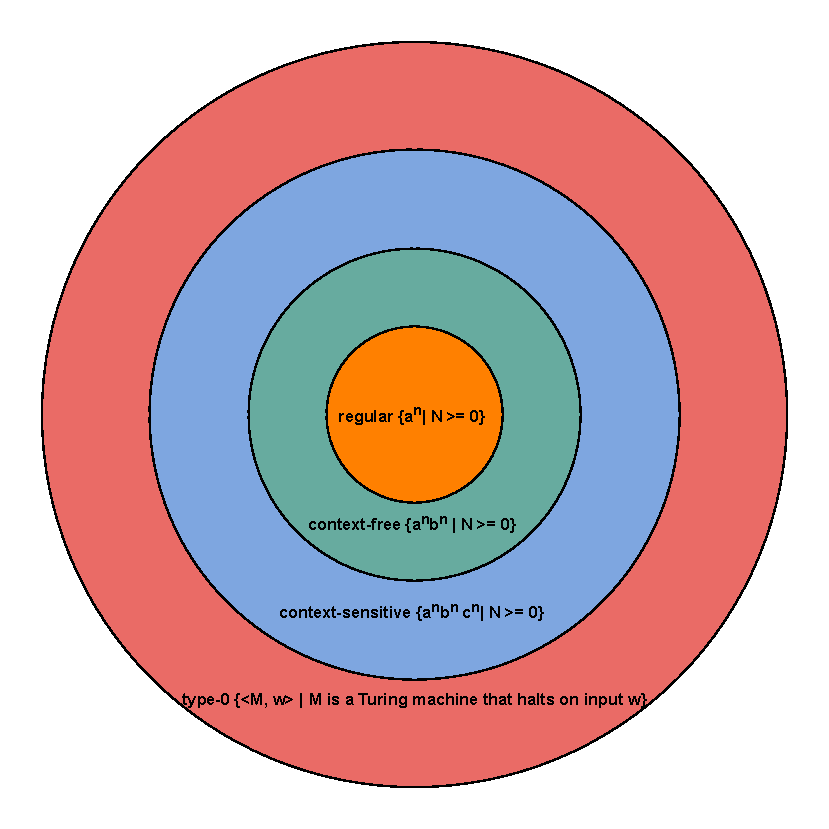
\includegraphics[scale=0.8]{obrazky-figures/chomsky.pdf}
    \caption{Chomsky hierarchy.}
    \label{fig:chomsky}
\end{figure}

\begin{theorem}
\label{teo1}
$$ \mathbf{FIN} \subset \mathbf{REG} \subset \mathbf{LIN} \subset \mathbf{CF} \subset \mathbf{CS} \subset \mathbf{RE}$$
\end{theorem}

\chapter{Music Theory, Musicology, and Their Properties}
\label{chap2}
The main topic of this chapter is to give a reader a basic understanding of what music is and what it takes to create musical peace. We will show what notation musicians and composers use in order to capture music. But not just that, we will dive really deep into music theory and reveal complex transformations that create music that is pleasing to listen to. We will discuss the music language and where it is located in the Chomsky hierarchy. We will explain the decision that led us to generate music using formal models. With that, we will reason with the formal model we used to create the music piece.

The basics of music theory in this chapter are form \cite{droppova1998}. I have used \cite{noteflight} to create music notation images in this chapter.

\section{Music art}
Let's talk about dominant and essential expressions in the sound structure of musical compositions, which are melody and rhythm. They create a foundation for perceiving and understanding the music we listen to, while they play a significant role in influencing its mood. Dominant musical expressions such as melody help to understand the main idea in various musical forms arranged in a specific order (motif, theme, sentence, etc.). In temporal space, we can find a rhythm that is tight and close to tempo, which highly influences the duration of the composition.

The next important expression in music is harmony. It is the basic building block of many compositions because it allows the composer to reach expressive contrasts of consonance and dissonance. As with melody, the effect of harmony is more enhanced when there is a specific rhythmic structure and growing dynamics.

The last one is the instrumentation, which gives a characteristic expression of the composition and tonal color. We want rich, diverse, and engaging musical compositions that are done with the orchestra, which has a large variety of musical instruments.

Understanding musical composition is not just about having knowledge of musical expressions. However, we have to have ability to emotionally engage with the music.

\section{Fundamentals of Sound and Tone}
In our daily lives, we encounter a variety of sounds. We hear birds singing, the noise of machines, the screech of a train, or the melody of musical instruments. Some of these sounds are pleasant, while others can be annoying. Examining these differences is very important from the perspective of music generation. We could dedicate entire chapters to this topic. However, we will cover at least the basics.

\subsection*{Sound}
Sound is a physical phenomenon that comes from the source of sound. It is created by the vibration of an elastic body. When this body starts to vibrate, the air around it starts to produce a wavy motion. Similar phenomena we see in nature, for example, when we throw a rock into the lake and see the waves spreading outward in all directions. There are four conditions that when they are satisfied, we hear sound:

\begin{itemize}
    \item{sound source -- elastic body -- string or membrane,}
    \item{trembling of the sound source -- hitting, rubbing and strumming,}
    \item{conductive environment -- atmosphere,}
    \item{auditory organ.}
\end{itemize}

\subsection*{Tone}
Tones are our noble sounds that are produced by the sound source and are created by the regular trembling of the sound source (e.g., singing, sounds from musical instruments). The irregular trembling of the sound source is called noise (e.g., rustling, thudding, rumbling). In music, we use both, but primarily, we want to produce tones. We define tone as a sound that has a certain height, which is created by regular vibrations from the sound source. Those vibrations are transferred to our auditory organs with the changes in compression and rarefaction of the air.

In our work, we will take into consideration three basic properties of a tone:
\begin{itemize}
    \item{pitch}
    \item{intensity}
    \item{timbre}
\end{itemize}

We can read the properties of a tone from a unique curve called the oscillation curve. A special property of a tone that is not physical property is tone length. This property depends solely on the musician or subject responsible for the tone's duration. If we have to pick the most essential properties, it would be pitch and duration.

The pitch of the tone is calculated by the number of vibrations per second. Higher tones correspond to a higher number of vibrations per second. This is expressed by the frequency, which is measured in Hertz. If we want to determine the frequency of a tone, we can do that in two ways. One is absolute, we specify the exact number for tone $a_1$, it is 440 Hz. It can also be done relatively. It is when we compare the pitches through intervals between two tones.

We see on the image \ref{fig:a1a2} the relationship between two tones that are distanced by one octave. The height of the tone $a_2$ is 880 Hz.

\begin{figure}[H]
    \centering
    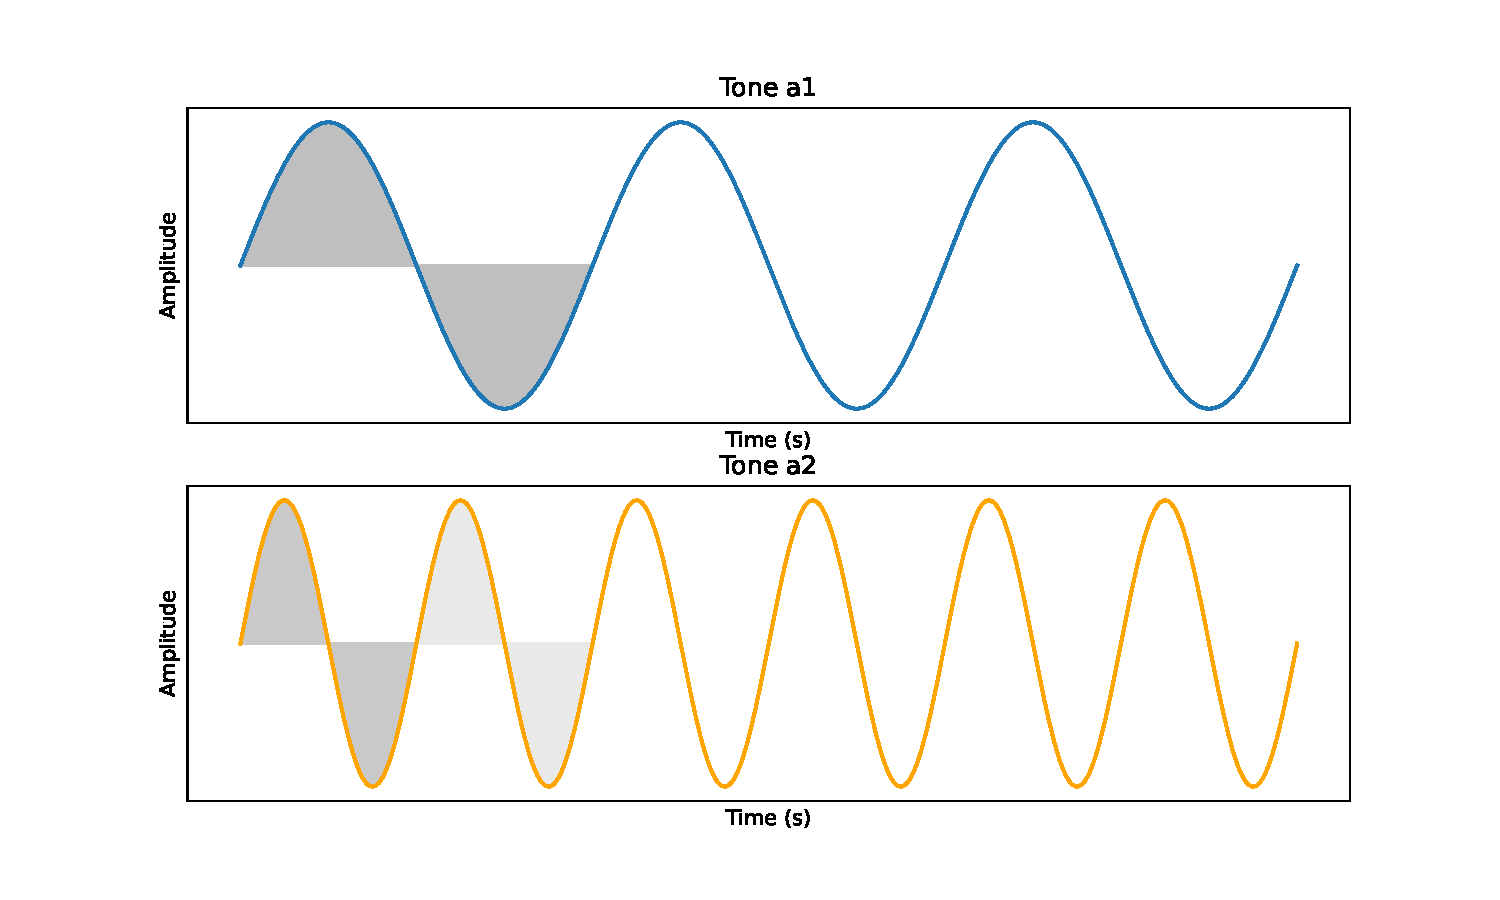
\includegraphics[scale=0.55]{obrazky-figures/a1a2tones.pdf}
    \caption{The difference between tone a1 and a2.}
    \label{fig:a1a2}
\end{figure}

The next important property is intensity. Intensity is closely related to the magnitude of the oscillation, or in other words, the amplitude, which represents the width of the vibration. As the width of the vibration in the oscillating device increases, the tone becomes more powerful. For a tone to be audible, it must fall within a certain frequency range, approximately from 20 Hz to 20,000 Hz—the range detectable by the human ear. The intensity of sound is measured in decibels (dB), which is the unit used to quantify sound intensity.

The number and intensity of the accompanying partial tones influence the timbre of a~tone. A string never vibrates only as a whole; its motion is divided into halves, thirds, quarters, and so on. This results in a compound tone; partial vibrations create that. This differs for every musical instrument.

The final property we will discuss is the duration of a tone. The length of the oscillation of the sound source determines it. The performer is the only one who can change the duration of a tone.

\subsection*{Representation of Music Through Notation}
Musical notation is a collection of graphic symbols, abbreviations, markings, and text expressions that are needed for documenting and interpreting musical ideas, melodies, or musical compositions. The tone properties that are noted in the music notation are the height and the length. They are written directly, we call them notes. Other properties that are noted need special characters.

Notes are written to the musical staff. It has five lines and four spaces. The Ledger lines are extra lines that could be added before or after the classic music staff. Music staff can be found in the picture \ref{fig:notes}. 

In the image, we see a note $c_1$, depicted in various durations, which are used throughout this thesis and implementation. Starting from the left, there is a quarter note, followed by a quarter rest. Next is a half note, accompanied by a half rest. The following note has the duration of an eighth note, along with its corresponding rest. Finally, there is a whole note with a whole rest.

\begin{figure}[H]
    \centering
    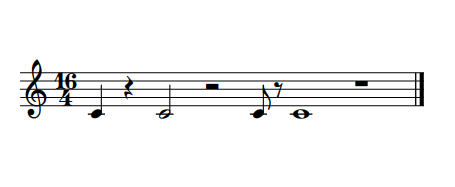
\includegraphics[scale=0.55]{obrazky-figures/notes.png}
    \caption{Basic Notes and Rests Chart.}
    \label{fig:notes}
\end{figure}

A rest plays a unique role in music and is almost as important as a note. With their help, we create contrast and interesting tension in music. This puts emphasis on preceding and following notes. Pauses can create a sense of anticipation and drama that adds more interest to the music.

\subsection*{Tonal organization in music}
Tonal organization in music is a set of all tones that are used in music. We recognize seven foundational tones that are arranged by the pitch and its names: c, d, e, f, g, a, h. There is no special name for the eighth tone because it is a repetition of the first tone but in higher pitch. Following tones are also in higher pitch and they are order in the same way. Those tones form an octave in the tonal system.

By an octave we can also mean the eighth tone of the original series of tones. This tone is specific because it has double the frequency of the first tone and produces a sound that aligns harmonically with it.

We have not talked about semitones. The semitone is the smallest distance between two tones in the tonal system. It cannot be divided. If we add two semitones, then we would get one whole tone. In case we want to increase the tone by semitone, we use sharp. If we want to lower the tone by semitone, we use flat. We see that in the music staff in the image \ref{fig:semitones}. Tone g in the first measure is increased by a semitone, and then tone g is lowered. The same was applied to tone a.

\begin{figure}[H]
    \centering
    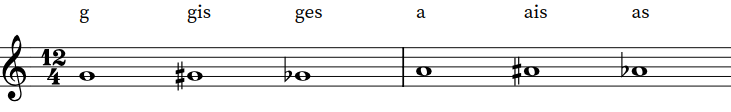
\includegraphics[scale=0.55]{obrazky-figures/semitones.png}
    \caption{Semitone examples for tone g and a.}
    \label{fig:semitones}
\end{figure}

We already mentioned measure. One measure is the basic unit of the alternation between strong and weak beats. By the strong beat, we mean the first beat in a measure. We separate measures with bar lines. The double bar at the end indicates the end of the music solo.

What determines how notes are organized into a measure is the time signature. It takes the form of a fraction, but without a fraction bar. In our example (\ref{fig:semitones}), the time signature is 12 over 4. The number 12, also called the numerator, represents the number of beats in a measure, while the denominator indicates the note value assigned to one beat. In this case, our measure can contain three whole notes, each lasting four beats. Alternatively, if we use quarter notes, which last one beat, we could fit twelve of them into the measure.

\section{Understanding Melody and Harmony}
As we move deeper into this chapter we should explore the concepts of melody and harmony. Melody is something that everyone can create or produce with his own voice while we whistling or singing. It is a sequence of single notes that are being sung one at a time. Our favorite songs contain pleasurable melodies that are sung or played.

Harmony, on the other hand, arises when multiple voices or sounds are played simultaneously. In our previous example, when two people whistle or sing together, they create harmony. Even if they sing out of tune or the sound grates on the ears, it still makes harmony.

In music, we commonly use multiple notes played together to create harmony. In this work, we will primarily focus on three tones sounding simultaneously, which are referred to as chords. In modern music, as we want to reproduce it as closely as possible, chords are commonly used, and they create a structural basis for an entire piece of music.

Usually, it is not in music in one way or another. Melody in music is enriched with specific chords that are played underneath it. An experienced composer or musician can see notes in a melody that suggest specific chords. A single chord can suggest notes for melody. What is really interesting and what we aim to do in this work is to combine sequences of chords. It should create melodies within the harmony. This approach produces a sound that most people find enjoyable to listen to.

The difference in notes could be found in the image \ref{fig:harmonicmelodic}.
\begin{figure}[H]
    \centering
    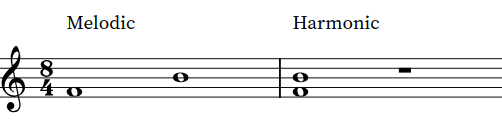
\includegraphics[scale=0.55]{obrazky-figures/harmonicmelodic.png}
    \caption{Semitone examples for tone g and a.}
    \label{fig:harmonicmelodic}
\end{figure}

\subsection*{Triads and Chords}
Triads are a specific type of chord, formed by a combination of three notes played together in structured intervals. In contrast, a general chord can consist of any combination of three notes, without adhering to a specific pattern or structure. We recognize multiple types of triads.

\begin{itemize}
    \item{Major triads are characterized by their bright and stable sound. They evoke happy, optimistic emotions in people. They feel warm and confident. To create a major triad, we have to start with any root note, and then we stack another note that is distanced from the first one by four semitones. The third stacked note is distanced by seven semitones from the root note. Major triads are considered to be the default. In our work, when we say C chord, then we mean C major triad.}
    \item{Minor triads are considered to be the opposite of major triads. They are often characterized as dark, somber, melancholic, or even ominous. It has a reversed structure of a major triad. It starts with a tone that is distanced by three semitones from the root. The last one is distanced by 7 semitones from the root. It is denoted by "m". So when we create C minor, we write Cm instead.}
    \item{Augmented triad is the least used triad from all four. It has some unique properties. It is often used as an elevator of chord progression. It is never used as a key component.}
    \item{Diminished triads are well known for their volatile and unstable nature. It is done by a tritone it contains. We can describe this triad as chaotic, harsh, and tense. }
\end{itemize}

In our work, we will use these types of chords. Later, we will talk about chord progressions. 

The harsh reality is that major chords can be easily mixed up together, and the music usually sounds good. Building a chord progression that we like requires us to experiment. It takes time to find an enjoyable sequence. For example, we have sequences that are used in popular music.

Certain chord progressions play a crucial role in popular music and are often tied to iconic compositions. 
For instance, the progression \textbf{A -- G -- C -- D} is prominently featured in Michael Jackson's \textit{"Stranger in Moscow"}. 
Similarly, the descending sequence \textbf{A -- G -- F -- E -- D -- C -- B} forms the outro of The Beatles' \textit{"I Am the Walrus"}. 
Another example is the progression \textbf{E -- D -- A -- G}, which serves as the foundation for the chorus in Buffalo Springfield's \textit{"For What It’s Worth"}.

To this day, there is no definitive explanation for why these chord progressions are effective. However, this has almost no consequence, as talented songwriters often create remarkable music without relying heavily on music theory. In practice, the knowledge of music theory often plays a secondary role to creativity and intuition.

Minor chords are less prevalent in music compared to major chords, as their sad, melancholic, and somber tones make them less suited for popular music. Instead, they are often combined with major chords to create more dynamic and interesting sounds. Despite their limited use in popular music, minor chords play an important role in specific contexts. They are frequently heard in horror, sci-fi, and Halloween-themed scenes, where their emotive quality enhances the atmosphere.

\subsection*{Chords and their contextual behavior}
We already know that major chords are bright, warm, and happy sounds, but this is not always the case. Major chords can be surrounded with notes that evoke different emotions like melancholy, fear, or uncertainty. This shows that major chords and chords, in general, are dependent on context. In a later section, we will have to take this into account and find a formal model that will handle this. An example of darker-sounding chords is in the figure \ref{fig:darkmajorchords}.

\begin{figure}[H]
    \centering
    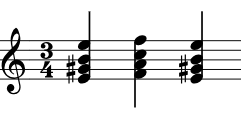
\includegraphics[scale=0.55]{obrazky-figures/chords.png}
    \caption{Example of darker major chords.}
    \label{fig:darkmajorchords}
\end{figure}

In our example, we use two major chords. The first is an E-major chord followed by the same chord shifted up by a semitone, resulting in an F-major chord. When we play this chord sequence it evokes dramatic emotions, which are not usually associated with major chords. That is the reason, we say that our interpretation and emotional experience is highly dependent on what precedes and follows them.

\subsection*{Chord progressions}
To get into the topic of chord progression, we have to talk about the leading tone. The leading tone is the 7th tone in any major scale. For example, the tone F\# in the G major scale has a special tendency to ring in our ears, it creates tension that makes us want more of the melodic story. After we play the tone above it, the tone G, the tension disappears. This commonly occurs in many compositions and is used by musicians within chord progressions, which makes the music more engaging.

\section{Neo-Riemannian Transformations and Tonnetz}
We have previously explored major and minor triads, we now aim to build upon this foundation by introducing a more advanced framework for understanding harmonic relationships: Neo-Riemannian transformations. These transformations provide a powerful tool for analyzing and generating chord progressions, particularly when exploring chromaticism and voice-leading beyond conventional contexts. Thanks to them, we can create smooth relations between chords.

All the information presented in this section is derived from the work in \cite{neo-riemannian, absil2025schillinger, mansonthesis}.

\subsection*{PLR family}

Work of David Lewin came with an idea that create operations between triads and create model that explains them. This was based on the idea from musical theorist Hugo Riemann. Following work that was builing on top of that was focused on three basic operations that maximize pitch-class overlap between pairs of distinct triads. Those operations were:

\begin{itemize}
    \item{Parallel (P) for triads that share the same fifth.}
    \item{Leading tone exchange (L) for triads that share the same minor third.}
    \item{Relative (R) for triads that share the same major third.}
\end{itemize}

An example of these operations represented on a music staff can be seen in Figure \ref{fig:cminorneoriemann}. The figure illustrates all three transformations applied to a C minor triad. In the first measure, the L transformation shifts C minor to As major. The second measure demonstrates the P transformation, converting C minor to C major. Finally, the third measure shows the R transformation, which changes C minor to Es major.

\begin{figure}[H]
    \centering
    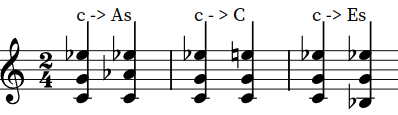
\includegraphics[scale=0.6]{obrazky-figures/Neoriemann.png}
    \caption{PLR transformations of C Minor.}
    \label{fig:cminorneoriemann}
\end{figure}

We can observe that each transformation inverts the chord's tonality, shifting from minor to major in our example. However, the process can also work in reverse, transforming a~major chord into its minor counterpart. If we apply these transformations twice, the chord's original tonality is restored, returning it to the same major or minor quality as it had before the transformations were applied.

The main feature of PLR family is that the operations create smooth and efficient voice-leading. Or, in other words, they are parsimonious. It is embedded so much that two consequent chords share two notes, and just the third note is changed. The third note is changed by a semitone in the case of P and L transformations. In the R transformation, the third note moves by a whole tone. This feature is deeply rooted in the evolution of musical styles that rely on stepwise voice-leading and semitonal motion in particular, have remained lasting standards across the musical history and styles. The parsimony of PLR-family voice-leading is so deeply rooted in the practical knowledge of musicians trained in~the European tradition that it often goes unnoticed.

\subsection*{Tonnetz}
Tonnetz, or a table of tonal or harmonic relationships, is a two-dimensional matrix and a~tool that can visualize chord progressions. This tool has a long history and is being used by music theorists to this day. At the beginning, the Tonnetz was designed to picture acoustic connections between chords and how they relate to each other. Late research showed that chords could be understood using mathematical structures, namely the group theory. With the help of group theory, we can systematically and mathematically describe movement between chords. Tonnetz also incorporates these group-theoretic relationships and shows that chords are not connected just by acoustic properties but also through mathematical transformations. A tool like this provides the possibility to connect to the mathematical description of this structure and, in turn, use formal models to control and generate harmonic progressions.

Throughout history, Tonnetz was modernized by multiple methods. At first, it was created to show the relationship between two specific intervals that form the foundation of minor and major chords. This was done by Euler. He designed a small finite grid, and later, Oettingen expanded this idea into the infinite grid. Finally, Riemann adopted this version and made it popular among German music theorists, and this is popular to this day. Historically, the Tonnetz was used to reinforce traditional tonal harmony, focusing on the Tonic, Subdominant, and Dominant (TSD) framework developed by Riemann. This approach overshadowed PLR-family operations, even though they provide a natural way to describe smooth transitions between chords. Modern theorists like Lewin and Hyer challenged this view, arguing that PLR transformations better capture the harmonic fluidity of Romantic-era music. 

We have discussed the history to understand what is capable of capturing the Tonnetz and how it remains relevant today. We will leverage these properties in our music generation. The Tonnetz is not limited to Romantic-era music; its properties can be found across the entire spectrum of classical music. To see what the Tonnetz actually looks like, refer to Figure \ref{fig:tonnetz}. The PLR relationship between notes from our example \ref{fig:cminorneoriemann} is also graphically shown in the graph.

\begin{figure}[H]
    \centering
    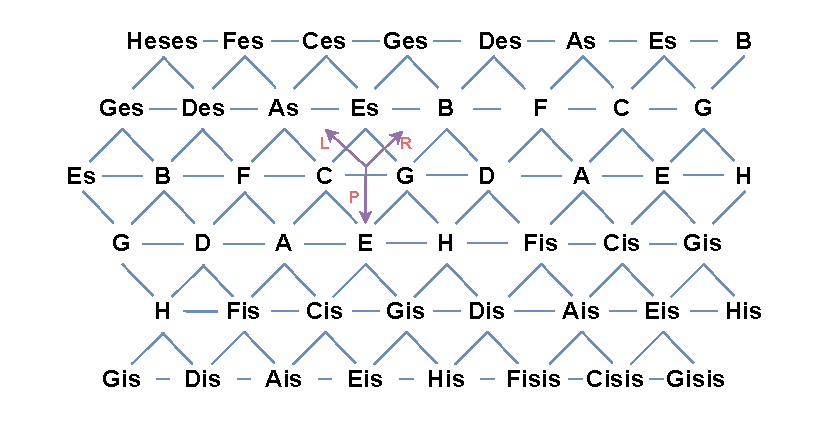
\includegraphics[scale=0.8]{obrazky-figures/tonnetz.pdf}
    \caption{Tonnetz diagram with pitch names.}
    \label{fig:tonnetz}
\end{figure}

Transformations between chords in the Tonnetz can not be applied twice, they are involutions. This means that we can find in it only major and minor triads and augmented and diminished triads are excluded. This helps maintain harmonic structure while allowing smooth and predictable transitions between chords.

The nodes in the diagram \ref{fig:tonnetz} are pitches that form triads. In our case example we had c minor (C, Es, G) with P transformation to C Major (C, E, G). L and R transformations are shown in the diagram in similar way.

\subsection*{Meaningful Cycles Inside the Tonnetz Diagram}
When we examine the literature, we find that the Tonnetz is often used to explore and create cycles through the repeated application of PLR transformations. Let us start with the most popular cycle and then we move to others.

The most well-known type of cycle is the LP/PL cycle. We haven’t yet mentioned that the Tonnetz is three-dimensional structure when it is fully taken into account. If we keep moving through the Tonnetz in a continuous loop with our transformations, we will eventually return to the starting point of the chord progression. 

\[
\begin{aligned}
LP: & \ \text{C Major (C, E, G)} \rightarrow L = \text{E Minor (E, G, B)} \rightarrow P = \text{E Major (E, G$\sharp$, B)} \\
    & \rightarrow L = \text{A$\flat$ Minor (A$\flat$, C$\flat$, E$\flat$)} \rightarrow P = \text{A$\flat$ Major (A$\flat$, C, E$\flat$)} \\
    & \rightarrow L = \text{C Minor (C, E$\flat$, G)} \rightarrow P = \text{C Major (C, E, G)}
\end{aligned}
\]

\[
\begin{aligned}
PL: & \ \text{C Major (C, E, G)} \rightarrow P = \text{C Minor (C, Es, G)} \rightarrow L = \text{As Major (As, C, Es)} \\
    & \rightarrow P = \text{As Minor (As, Ces, Es)} \rightarrow L = \text{E Major (E, Gis, B)} \\
    & \rightarrow P = \text{E Minor (E, G, B)} \rightarrow L = \text{C Major (C, E, G)}
\end{aligned}
\]

How such a cycle appears in a diagram is shown in Figure \ref{fig:tonnetzLP}.

\begin{figure}[H]
    \centering
    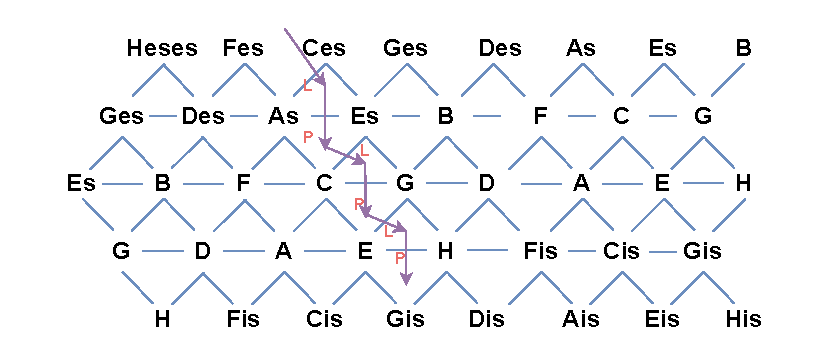
\includegraphics[scale=0.8]{obrazky-figures/tonnetzLP.pdf}
    \caption{LP cycle in the Tonnetz diagram.}
    \label{fig:tonnetzLP}
\end{figure}

This cycle was an important element in the compositions of composers such as Wagner, Franck, Liszt, Mahler, and Richard Strauss.

Another commonly used cycle is the PR/RP cycle. It creates music with more dramatic elements and greater contrast compared to the PL/LP cycles. Additionally, it involves a~larger harmonic collection, containing 8 pitch classes as opposed to the 6 pitch classes in~the PL/LP cycle. The example of such a cycle is shown below.

\[
\begin{aligned}
PR: & \ \text{C Major (C, E, G)} \rightarrow P = \text{C Minor (C, Es, G)} \rightarrow R = \text{Es Major (Es, G, B)} \\
    & \rightarrow P = \text{Es Minor (Es, Ges, B)} \rightarrow R = \text{Ges Major (Ges, B, Des)} \\
    & \rightarrow P = \text{Ges Minor (Ges, Heses, Des)} \rightarrow R = \text{A Major (A, Ces, E)} \\
    & \rightarrow P = \text{A Minor (A, C, E)} \rightarrow R = \text{C Major (C, E, G)}
\end{aligned}
\]

The last cycle is the LR/RL cycle, which is unique in that it includes all possible consonant triads. However, a complete LR cycle is too long to be considered a practical choice for use in a composition. But this does not stop composers from using it. Parts of this cycle are frequently used. Notable examples include Beethoven’s Ninth Symphony and Wagner’s Parsifal.

\subsection*{Compound PLR Transformations}
We have already introduced our PLR transformations, which allow for smooth transitions between triads. However, we have not yet discussed how PLR transformations can be combined to create unique progressions while preserving this smoothness. Compound transformations were widely used by many composers of the Romantic era. Cycles that were discussed previously have their place in theory and in small parts of compositions. Transformations have a broader reach in different genres. An excellent example of this can be found in Pop-Rock music, as discussed in the previously mentioned thesis \cite{mansonthesis}. An application of compound transformation RP can be found in Figure \ref{fig:tonnetzRPcombined}.

\begin{figure}[H]
    \centering
    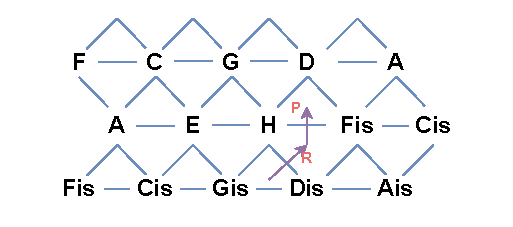
\includegraphics[scale=0.9]{obrazky-figures/tonnetzCompound.pdf}
    \caption{RP compound transformation.}
    \label{fig:tonnetzRPcombined}
\end{figure}

\[
\begin{aligned}
RP: & \ \text{Gis Minor (Gis, H, Dis)} \rightarrow R = \text{Dis Major (Dis, Fis, H)} \\ 
& \rightarrow P = \text{H Minor (H, Fis, D)}
\end{aligned}
\]

The properties of compound transformations differ from those of individual transformations. Unlike individual transformations, they are not involutions. To return to the original triad, the opposite compound transformation must be applied. Other combinations of the two can be obtained and applied.

We can also create and use a compound of three single transformations. For example, let us take E Major (E, H, Gis) to get H Minor (H, D, Fis). How we would do that is shown in Figure \ref{fig:tonnetzPRL}.

\begin{figure}[H]
    \centering
    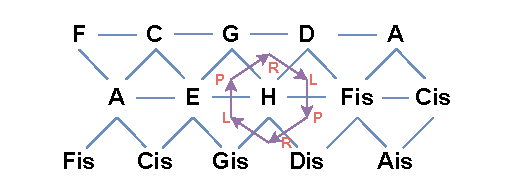
\includegraphics[scale=0.9]{obrazky-figures/tonnetzPRL.pdf}
    \caption{PRL compound transformation.}
    \label{fig:tonnetzPRL}
\end{figure}

The transformation of PRL compounds is special because it has involution. This property is demonstrated in our figure.

\section{Computational musicology}
Part of this work is also research on how to formalize our picked-up knowledge of music. We have covered and studied various types of languages and grammars. We have also covered the basics of music theory and some advanced topics that could build and analyze a structure in music. With this knowledge, there is the last important thing before we choose the right language model to generate or analyze music. We have to look at the structure of the music from a computational point of view. This topic is covered in \cite{musicformallanguage}, from which we used information that is in this chapter.

Many people, including \cite{musicformallanguage} argue that music language falls into the same class as natural languages do. This class is called mildly context-sensitive languages. As we discussed various properties that could be found in music, the classification in terms of the computational capacity of those parts also differs.

\section{Generative Capacity}
To start formalizing music, we have to talk about what weak and strong generative capacities are. When we just talk about string outputs that are generated by grammar, it is called weak generative capacity. If we take a closer look at complete derivations and the way the strings were generated, we talk about strong generative capacity. For us, it is much more interesting to focus on strong generative capacity as it gives us a more inside view of how formal models generate music. The hierarchy of formal grammars and languages was introduced in \ref{sec:chomhierarchy}. Within this framework, the language of music can be analyzed to determine its placement.

\subsection*{Regular Languages (Type-3)}
Regular languages are largely equivalent to regular expressions, which are commonly utilized in numerous UNIX tools and utilities. They have low computational complexity, they can be analyzed in linear time, and we can apply on them almost all algebraic operations. When it comes to music, they have limited generative capacity. Not that many parts or structures in music could characterized by regular grammar as we will later see.

Some attempts have been made to connect regular languages with Shannon n-grams \cite{musiclanguageanimals} under the condition that we forget the probabilities. Shannon's n-grams are commonly used in linguistics, and they model sequential structure in language. We define by them the probability of generating the next symbol in sequence in terms of the previously generated $(n - 1)$ symbols. An equal approach is used in music.

We will not dive deep into tree languages, but an example can be found in \cite{africathesis}. This work uses regular tree grammars and tree transducers to form a musical piece. The system begins by creating an initial tree and applies various tree operations to transform it.

Also, a small mention of music generated by regular grammar is in \cite{gramimprovisation}, but no modern works are built around regular grammars.

\subsection*{Context-Free Languages (Type-2)}
Context-free languages are characterized mainly by tree structures. An example could be a balanced pair of parenthesis or mirror structures. They find usage in programming languages as most belong to deterministicly parseable subsets of type-2 languages. Type-2 languages could be parsed in $\mathcal{O}(n^3)$ time. However, some challenges come with them, such as ambiguity, and they are not closed under complement or intersection.

\begin{figure}[H]
    \centering
    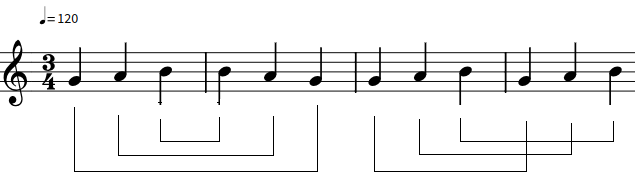
\includegraphics[scale=0.5]{obrazky-figures/mix-dependencies.png}
    \caption{Context-free and non-context free dependencies.}
    \label{fig:mixdepen}
\end{figure}

Specific music parts belong to this category, as shown in the first two measures in figure \ref{fig:mixdepen}. It is a simple melody when the first three tones rise in melody and the other three decline.

Many works in computational musicology are based on context-free grammars. From a formal perspective, one notable approach involves the use of probabilistic context-free grammars. One of them is \cite{probmelodyreduction}. We will talk about how this grammar is applied in music later.

Another example of type-2 grammar could be attribute grammar in \cite{controlflow}. But those grammars are used for something different than music creation and avoid structures we want to represent.

\subsection*{Context-Sensitive Languages (Type-1)}
This group of languages is usually described as a copy language. When we directly take a look at an example in music in figure \ref{fig:mixdepen}. Those last two measures are copies of each other. Such a language is decidable but computationally complex. From our small example, there is doubt that if we want to generate music, context-free options are enough.

An example of a work that uses context-sensitivity and its properties is presented in \cite{belproc}. This work focuses on tabla music, though the knowledge can be applied to other types of music as well. Regular grammar is straightforward and easy to use; however, it becomes uncontrollably complex when accounting for irregularities in actual performances. Not only that, but we want to work with jazz music that is mostly improvisational, and this would only compound the problem.

Our target in music analysis and generation will be classical and jazz music. It is the most effective way to demonstrate the power of music generation by formal models because this music contains structure. We have shown an example of structure in \ref{fig:mixdepen}. But there are more examples to come. One could be a variation of a motif in music that can be expressed by copy language. Another could be multiple musical instruments playing together in harmony. This interplay of numerous musical instruments is dependent on each other. We could also consider this as an example of context dependencies.

\subsection*{Recursively Enumerable Languages (Type-0)}
The last category that will not be needed, but we still mention it to ensure completeness, which are type-0 languages. These are accepted by Turing machines, equivalent to unrestricted grammars, and are generally considered synonymous with the set of computable functions. While Type-0 formalisms are extremely powerful, they are notoriously intractable. This is a property that we don't want in music.

\chapter{Related Work}
\label{chap3}
In the field of computer music, numerous methods exist for generating music. To better explain and show why our model is unique compared to existing approaches, we have decided to put together this chapter. There are many models in the field of computer science, and it is not hard to pick one and create a simple melody. But as we dive deeper into the music and what is behind it, this task is getting more difficult, as well as a way to interpret music generated by specific models.

\section{Lindenmayer Systems}
One of the most popular formal models used to generate music is the L-system. The paper that initiated further advancements in the usage of this model is \cite{lsystems1}. The use of L-systems was intended to explain the development of living organisms formally. This was studied by theorists from many scientific fields. Later, this was also applied to generate plants and trees. The author of the already mentioned paper found another application that was in~fractal curves. But this is not that interesting to us as the newfound application in~music that is generated by algorithms focused on musical scores. In this work, music scores are not generated directly. It believes that the graphical interpretation of the L-system is closely related to the interpretation of music. The generated string is parsed for a turtle that is driven by encoded commands in this string. A drawn Hilbert curve is navigated through, and horizontal line segments are converted to notes. Vertical line segments of this curve are used as pitch, and segment length determines the note duration.

\begin{figure}[H]
\centering
\hfill
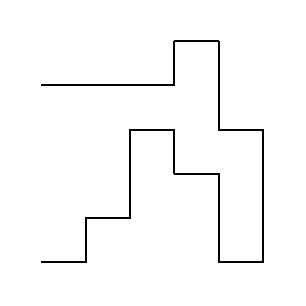
\includegraphics[scale=0.8]{obrazky-figures/lsys.pdf}
\hfill
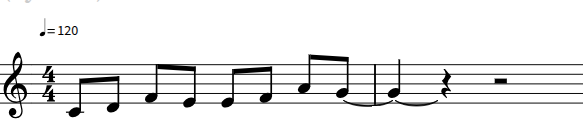
\includegraphics[scale=0.4]{obrazky-figures/lsys.png}
\hfill
\caption{A small example of the conversion of the Hilbert curve into music scores.}
\label{lsysturtle}
\end{figure}

An example of the algorithmic approach mentioned is in Figure \ref{lsysturtle}. Conversions start at tone C, and the curve transformation starts at the bottom left corner. A small example of the conversion of the Hilbert curve into music scores.

An interesting example of growing music can be found in \cite{lsystemsmix}. This work focuses on creating synchronized and aesthetically pleasing graphical and musical renderings. It explores various types of L-systems, with particular attention to the stochastic version, which is used to generate plant structures from the same family but with varying details. A similar concept can be applied to music, particularly when examining structured genres such as jazz or classical music. Defining a formal model that captures the characteristics of a stochastic genre variation could help generate diverse musical compositions. The second model used in this work is the context-sensitive L-system. The advantages of this model are that it allows to change the structure with respect to surroundings. This is useful in music for creating compositions where intensity, volume, or complexity increases. Of course, it could be used in other way around to simplify, soften, or reduce complexity.

\begin{figure}[H]
\centering
\hfill
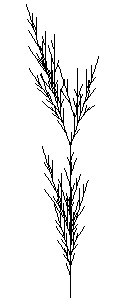
\includegraphics[scale=0.8]{obrazky-figures/cslsa.jpg}
\hfill
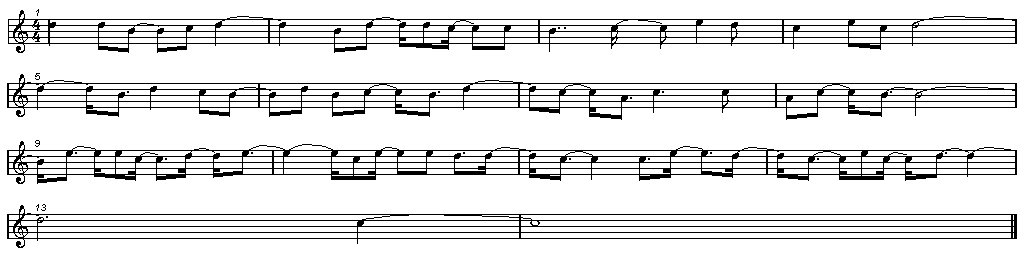
\includegraphics[scale=1.4]{obrazky-figures/cslsascore.jpg}
\hfill
\caption{Melody generated by stochastic L-system.}
\label{lsysstoch}
\end{figure}

An example of music generated by \cite{lsystemsmix} is shown in Figure \ref{lsysstoch}. This demonstrates a~simple melody that reminds the jazz solo inspired by a plant in the left part of this figure. This example and others used in the mentioned paper are in the depth of 3 or 4 iterations. This was proven to be the depth that creates interesting short melodies. With increasing iterations, melodies do not bring anything new and get dull. This should be solved by a~stochastic model. Using more interesting grammars like parametric L-systems can generate complex and realistic music. Additionally, the L-system that incorporates inputs from the environment could serve as inspiration. There are many ways to adopt this idea. One could be two L-systems reacting to each other while they generate their music.

The previously mentioned methods generate music but do not do so directly. They use some sort of postprocessing on the string that is being generated by a L-system. An~example that directly generates music could be \cite{straightlsys}. An improvement brings the work of \cite{bachelorthesis} where the author, compared to the previous paper, uses stochastic and context-free L-systems to experiment with direct music composition.

A complex dynamic system built on the hierarchy of L-systems that are connected to each other in a net structure is found in the work \cite{manousakis2006musical}. In addition to building such a~system, this work explores the possibility of interaction with an instrument or musician using L-systems. If we talk about the interactive system, then this work uses L-systems to segment and process incoming sound commands. However, the focus of this work is on the creation of a musical spatial domain. This domain is created by multiple L-systems, where each system generates a specific music element. Then, the next step is to map the resulting spatial space into music. That is done by a turtle that takes instructions that were created from the vector. The mentioned turtle moves in 3-dimensional space and can be considered to be a timed automaton. An example of this system is shown in Figure \ref{fig:lsystems}.

\begin{figure}[H]
    \centering
    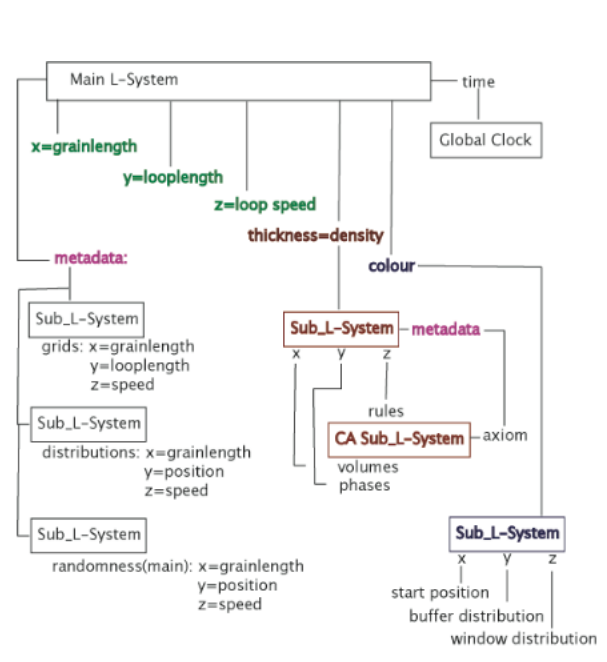
\includegraphics[scale=0.5]{obrazky-figures/lsystems.png}
    \caption{Hierarchy or L-system network.}
    \label{fig:lsystems}
\end{figure}

A different viewpoint on music in multidimensional space comes from \cite{gogins}. This approach uses simple operations to navigate through voice-leading and chord spaces. It is a~demonstration of a score generator based on L-systems that works in mathematical spaces that contain fundamental musical structures. Voice-leading is expressed as an orbifold with chords represented by points. The roughness of chords is modeled by the short distances of orbifolds. The closer they are, the smoother the voice. We have already discussed what Tonnetz is, as it is the primary driver of our score generation. This was inspired by this work as it uses Tonnetz to explain voice-leading connections between minor and major triads to find natural pathways between harmonies. Again, this work uses the L-system to produce commands for the turtle program, which is then converted to music.

\begin{figure}[H]
    \centering
    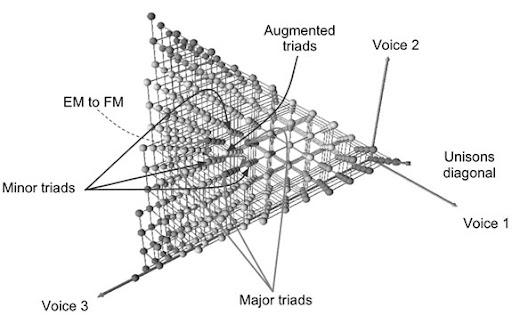
\includegraphics[scale=0.35]{obrazky-figures/trichordspace.jpg}
    \caption{Tonnetz for trichords.}
    \label{fig:goginstrichord}
\end{figure}

Figure \ref{fig:goginstrichord} illustrates how such a space can look. This illustration is taken from a modern book \cite{tymoczko2010geometry} that takes a look at music from a geometry point of view.

\section{Other Grammars}
We have covered one large group of models used in music generated by formal models. The next large group and maybe the last is probabilistic context-free grammar (PCG). Prime examples of this are works \cite{gramimprovisation}, \cite{probmelodyreduction}, and \cite{africathesis}. 

It was shown by \cite{gramimprovisation} that PCG could be used in tools that assist in creating jazz solos in the context of specific chord progressions. There are many ways to do this. One is manually creating a large database with different chord progressions. To avoid this, we need software that can dynamically generate melodic phrases that sound coherent and stylistically appropriate. To make such a software work, we need a PCG that makes notes fit into a melody, which is pleasing to listen to. Compared to different works, this one gives agility for a user to control specific constraints in grammar like minium and maximum pitch values, intervals, or probability to cross specified intervals. Another specificity is the categorization of terminal notes into chord tones, color tones, approach tones, and others.

On how to apply CFG to Bach Chorale melodies, we have to take a look at \cite{probmelodyreduction}. What they do is melody reduction to find the underlying structure of a melody or employ this model to generate melodies. They look at music as a high-level structure and consider it to be something much more than just a sequence of events. This work aims to provide a~definition of a statistical model of music that is compact and computable and brings more computational power than finite-state approaches. Because of that, no preference rules are used in grammar that could be preferred by listeners.

An interesting example of how to use tree grammars in music composition is \cite{africathesis}. They play with the idea of music generation with tree languages. Formal models used for this are regular tree grammars (RTG) and tree transducers. Regular tree grammars are used to generate the initial tree and then are applied transducers to form the final musical composition. The problem with this is that they can create only music with one voice. Like many other works, they are focused on specific styles of music, and they try to train models with this assumption. They use a combination of rules and statistical methods. This combination is divided into several different operations and reduces state space and processing power needed for each generation step. With that, the number of unique melodies that can be generated increases. The final formal models used in this work are also hidden Markov models, and they also experiment with variants like mixed-order Markov models.

\begin{figure}[H]
\centering
\hfill
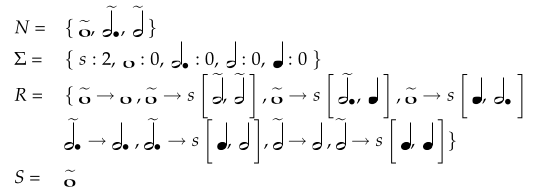
\includegraphics[scale=0.5]{obrazky-figures/Rhythmicafrica.png}
\hfill
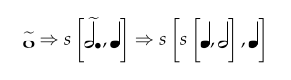
\includegraphics[scale=0.5]{obrazky-figures/Rhythmicafrica1.png}
\hfill
\caption{RTG and its rhythmic derivation.}
\label{africartg}
\end{figure}

Figure \ref{africartg} taken from \cite{africathesis} is a small example of how a small rhythmic phrase could be generated by RTG.

\section{Grammar in music notation}
Another area of music where formal models could be applied is music notation. We have talked mostly about music generation, but formal models could verify music notation as it is in \cite{controlflow}. This work is focused on control flow in score notation. Figure \ref{fig:controlflow} shows a~small example of control flow. In short, the notations Fine denotes the end of the music composition and D.C al Fine states that the composition should be played again from the start till the Fine label.

\begin{figure}[H]
    \centering
    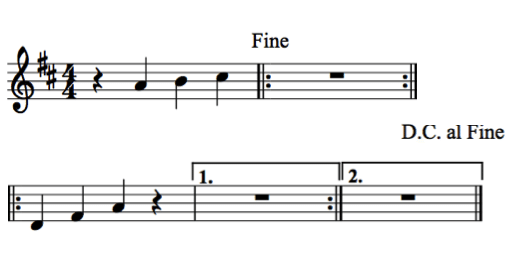
\includegraphics[scale=0.3]{obrazky-figures/notation.png}
    \caption{Control flow notation.}
    \label{fig:controlflow}
\end{figure}

The mentioned formal framework is based on context-free and attribute grammars. This combination guarantees that the interpretation of music notation is well-defined and unambiguous. The goal of context-free grammar is to create a parse tree that represents the from of final scores. Context-free grammar does not represent the meaning of music score by itself. For that, there is attribute grammar, which defines timing, duration, and repetition rules. This grammar enforces unambiguous representation and presents a flattened playable sequence of scores.

Frameworks like this find usage in computer-aided music processing. They enable tools like notation software, AI music systems, and digital performance tools to correctly interpret and execute musical scores with complex control flow elements.


\section{Music Automaton}
So far, we have been talking about grammars and their applications in music. An example of automata used in modern music is \cite{automataphd}. In this chapter, we have talked about many models that work in non-interactive environments. They create music in multiple steps. An idea that has not been mentioned yet is that we can use formal models to interact with its inputs. The example mentioned proposes a special framework that is able to create variable-form improvised pieces in real music performances. This is based on the framework of Rhythmically-Controlled Multi-Mode Audio-Based Interactive System proposed by \cite{automataphd}. The problem that is trying to solve this thesis is in recent developments in the field of interactive music systems that are fighting with rhythm issues. Formalization is done with the help of the theory of synchronized automata, which is enhanced with three structures. This defined concepts of mode and meta-mode.

Mode and meta-mode are terms that cover a structured way of controlling musical improvisation in interactive music systems using automata theory. Mode is a specific state of the system during musical interaction. Meta-mode takes care of the interaction between modes and manages when and how to switch modes. Those are the key aspects of developing reasonable and rhythmically driven systems used in live performance.

\begin{figure}[H]
    \centering
    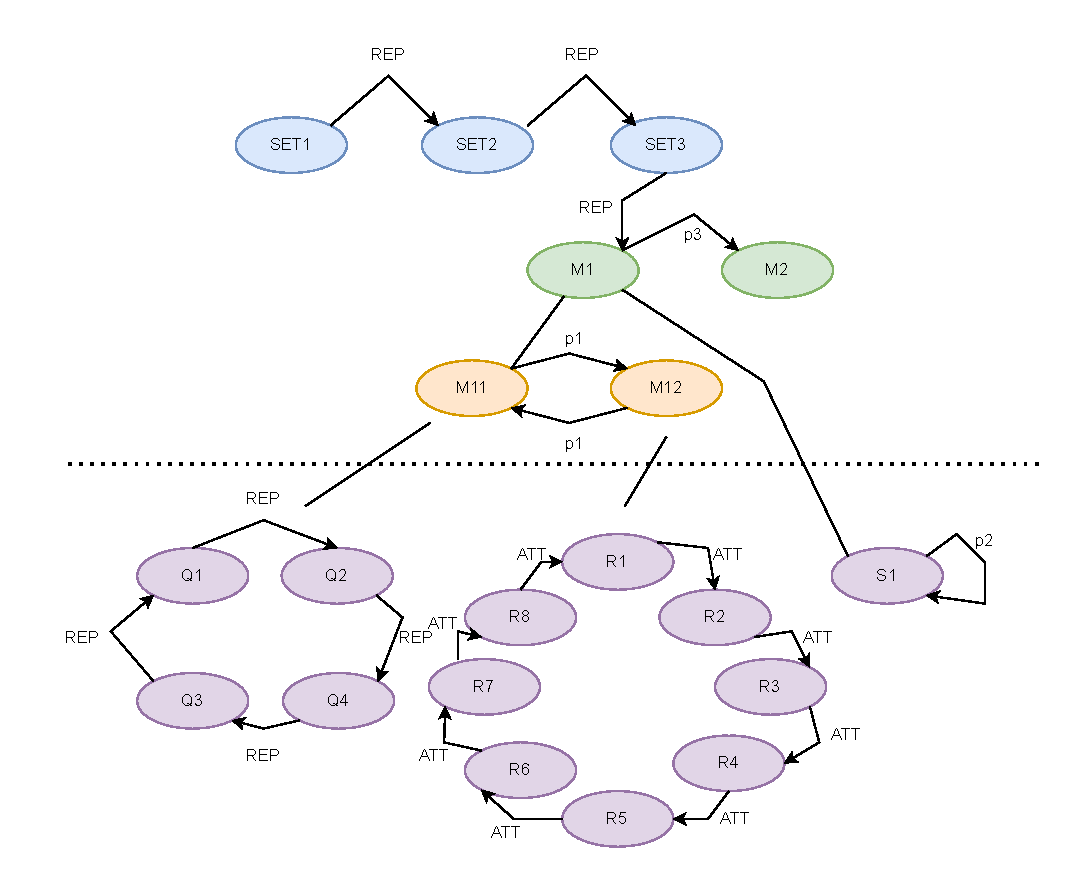
\includegraphics[scale=0.6]{obrazky-figures/automaton.drawio.pdf}
    \caption{Rhytmically-Controlled automata.}
    \label{fig:automataphd}
\end{figure}

Automata in figure \ref{fig:automataphd} is in initial state $(Q_1, R_1, S_1, SET_1, M_{11})$. This system has a tree structure. The dotted line divides this system into meta-modes and modes of interaction. Meta-modes are above the line, and modes are below. Each automaton is driven by different actions. REP is to detect repetitions of rhythmic phrases. ATT is an action made after an attack. Detection of the phrase is denoted by $p$. Detailed description on how this work could be found in cited work. Another interesting thing is that this work uses input sound waves to make actions. It applies knowledge from signal processing theory.

\chapter{Design and Application of Computational Models}
\label{chap4}
Finally, we will present further advances in the field of Musicology. This chapter will show how a music with great formal structure can be generated with a proper selection of formal models. We have chosen to use scattered-context grammar to capture various cross-dependencies in music. The related work we studied did not mention how formal models can generate multi-instrumental music. To address this gap, we propose the use of a multi-generative grammatical system as the most suitable approach. In this chapter, we give the reasoning behind all of those decisions and show the applications for those models.

Some parts of this chapter are related to my bachelor's thesis \cite{jozef}. Popular chord progressions were taken from \cite{justinguitar_chord_progressions} and used in provided examples to demonstrate music generation. I have used \cite{noteflight} to create music notation images in this chapter.

\section{Model Definition}
The presented section introduces a definition of a formal model that can generate classical music for multiple instruments. This model builds up on multigenerative grammar systems defined in \cite{LanguageTheory} and \cite{Lukas2006}. The uniqueness of this system is that it allows grammatical components to apply its rules in a single generation step. When this generation process stops, the generated strings in the model are put together using one of the string operations. But this is not something we want as we want to keep those generated strings for specific instruments to be played. For a positive integer $n$ our $n$-generative grammar system works with $n$ scattered grammars, which represent cross-serial dependencies in music. In our case, the number $n$ is the number of staves in a musical composition. As an example we can use piano-violin sonata written on a three-stave system, with two staves for the piano (right and left hand) and one for the violin. Grammar as components of the system do derivation steps concurrently to ensure mutual interconnection, where both instruments play music and complement each other. This is managed by the finite set of $n$-tuples of rules. When the derivation process is done, then there are $n$ strings of notes for selected instruments to be interpreted.

Below, we present the formal definition of this system, detailing its grammar rules, derivation process, and interaction mechanisms.

\begin{definition}
\label{Defnmgr}
An n-generative rule-synchronized music grammar system is defined as an $(n+1)$-tuple $$\mathbf{G_s} = (G_1, G_2, G_3, ..., G_n, Q),$$ in which

\begin{itemize}
    \item{$G_i = (N_i, T_i, P_i, S_i)$ is a scattered-context grammar introduced in Definition \ref{Def21}, for all i = 1, ...., n;}
    \item{$Q$ is a finite set that consists of n-tuples structured as $(p_1, p_2, ..., p_n)$, where $p_i \in P_i$, for all i = 1, ..., n.}
\end{itemize}
\end{definition}

In addition to the original definition, we will use tokens instead of plain terminals. Tokens have indexed attributes they represent that are going to be taken into account in~the final music interpretation by the instrument. Tokens are in the form $t_{[w_1, w_2, ..., w_n]} \in T_i$, where $w_1, w_2, ..., w_n$ are music attributes like tone length, special operation (tone inversion, shift, etc.), chord or others.

To improve readability while generating harmonic passages in music, we chose to represent chords using symbols from the Greek alphabet for simplicity, as they are difficult to denote with single-character symbols. In our examples, we will have tables that map Greek symbols to chords.

The final strings derived from the start symbol of a grammar or in our model are in~$n$-form as $n$-tuples structured as $S_f = (x_1, x_2, ..., x_n)$, where $x_i \in (N \cup T)^*$, for all $i$ = 1, ..., $n$. Let us take
$$c = a_1A_1...a_nA_na_{n+1},$$
$$d = a_1x_1...a_nx_na_{n+1}.$$ Then $S_f = (c_1, c_2, ..., c_n)$ and $\bar{S}_f = (d_1, d_2, ..., d_n)$ we consider to be sentential $n$-forms, in~which $c_i,d_i \in (N \cup T)^*$, for every $i$ = 1, ..., $n$. Consider $r_i$: $(A_1,...,A_n) \rightarrow (x_1,...,x_n)$ $\in P_i$ for all $i$ = 1, ..., $n$ and $(r_1, r_2, ..., r_n)$ $\in Q$, such that $c_i \rightarrow d_i \in r_i$. Consequently, $S_f$~directly derives $\bar{S}_f$ in $G_s$, denoted by $$S_f \Rightarrow_{G_s} \bar{S}_f.$$

Let us generalize $\Rightarrow_{G_s}$ with $\Rightarrow_{G_s}^k$, for all $k \geq 0$, $\Rightarrow_{G_s}^+$ and $\Rightarrow_{G_s}^*$. Generated $n$-string of $G_s$, denoted by \textnormal{n-}$S(G_s)$, we define by $$n\textnormal{-S}(G_s) = \{(w_1, w_2, ..., w_n) | (S_1, S_2, ..., S_n) \Rightarrow_{G_s}^* (w_1, w_2, ..., w_n),$$ $$w_i \in T^*, \textnormal{for all} \, i = 1, ..., n\}.$$
% jozef
\section{Encoding Musical Concepts into the Grammar}
Music has structure, and there are many attempts to formalize it. Our focus is mainly on well-known music genres that are recognized for their structure. But not just those genres have structure, but many others, like popular songs. To showcase our model, we have picked the sonata form from classical music, and jazz music is represented by its standard form. The mentioned forms presented here are taken from \cite{ravelliJazzForm2025} and \cite{Kadlec2022}.

We have two simple examples in figure \ref{fig:jazzclassic} that will be used to demonstrate how musical pieces could be encoded into grammar. On the left side, we have the popular jazz song Take The A Train taken from \cite{ravelliJazzForm2025}. The right side of the figure \cite{PankhurstSonataForm} shows a minimalistic example of sonata form called Allegro in F composed by Mozart.

When choosing a top-down approach to analyze a musical piece, we start by examining its overall structure. A great example is the jazz song shown in Figure~\ref{fig:jazzclassic}, which uses the most common structure in jazz standards, the AABA form. This song consists of two distinct sections (A and B), with each section typically spanning eight measures. These sections form the standard 32-measure framework of the basic melody found in AABA jazz compositions. 

\begin{figure}[H]
\centering
\hfill
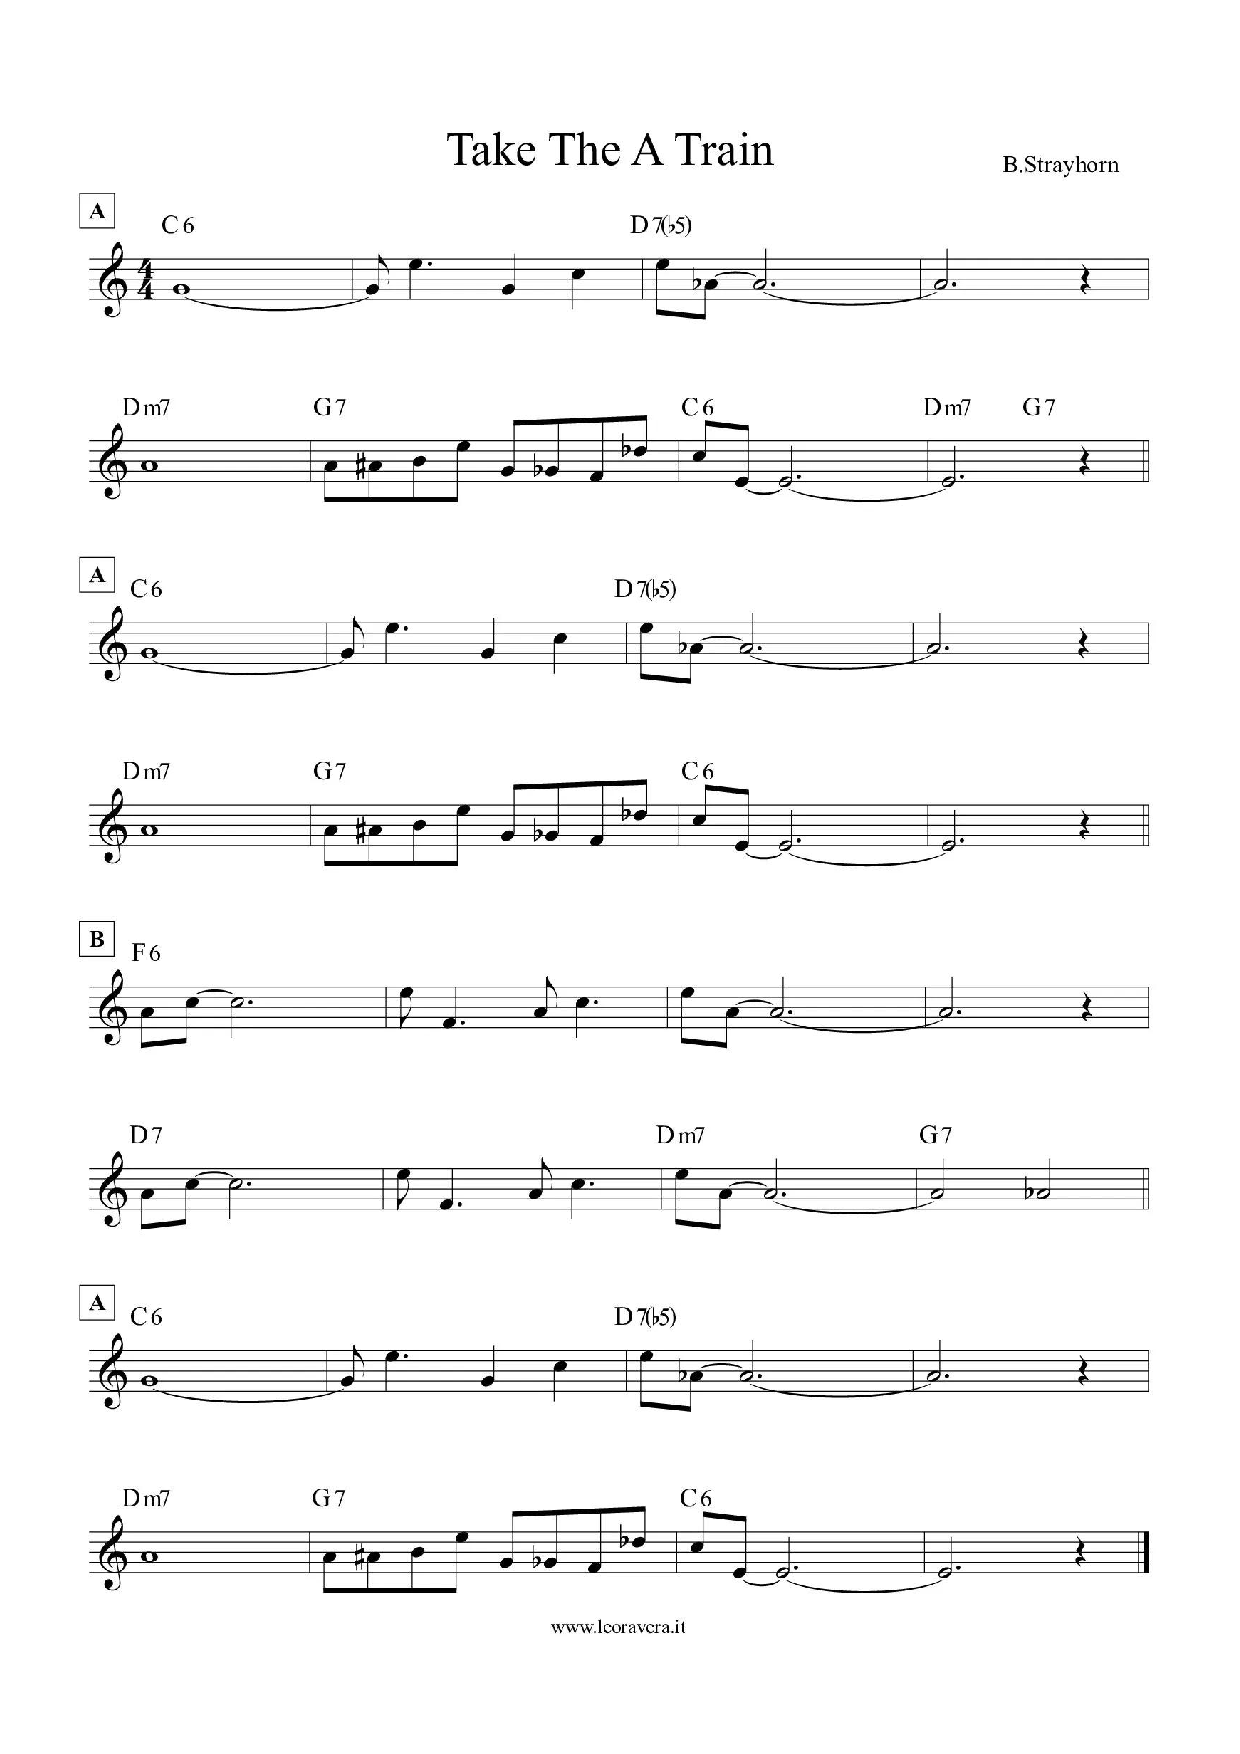
\includegraphics[scale=0.32]{obrazky-figures/Take-the-A-train-Billy-Strayhorn.pdf}
\hfill
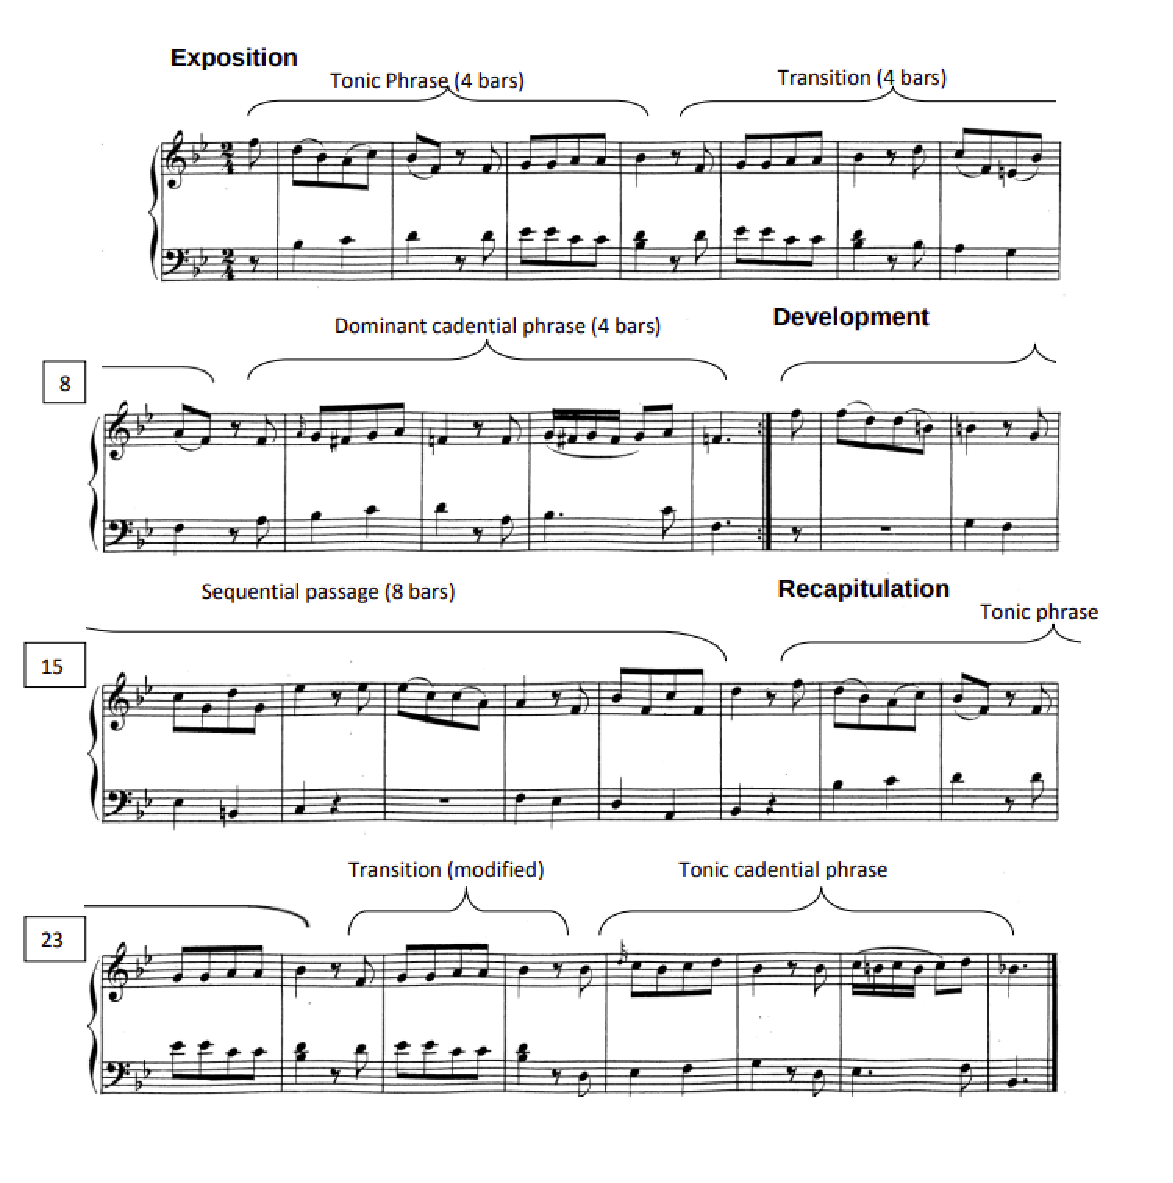
\includegraphics[scale=0.42]{obrazky-figures/sonataform.pdf}
\hfill
\caption{Jazz form (the left side) and sonata form (the right side).}
\label{fig:jazzclassic}
\end{figure}

When applying a similar analytical approach to the sonata form, we observe a three-part structure: exposition ($A$), development ($B$), and recapitulation ($A'$). The exposition introduces the primary thematic material, typically divided into two contrasting themes. The development explores these themes through variations, modulations, and transformations. Finally, the recapitulation returns to the original thematic material, usually restating the exposition themes in their original keys or slightly modified. This structured approach allows composers to achieve a coherent and varied musical narrative, which is fundamental to classical sonata compositions.

To achieve mentioned music forms it is a great idea to generate them using start symbols as an example could be 
\begin{align*}
S &\rightarrow AABA \\
\text{or} \quad S &\rightarrow ABA'.
\end{align*}.

But in the end, it is up to the composer to choose the form he wants his music to be in.

\subsection*{Encoding Melody and Harmony}
Once we have generated the initial nonterminals that outline the structure of the musical piece, the next step is to create the actual musical content. Music is truly creative, and there are endless possibilities. In our sonata example, we could encode exposition into three non-terminals $T_1, R, T_2$ and similarly recapitulation $T'_1, R', T'_2$. The symbol $R$ represents the transitions between the tonic and dominant phrases $T_1$ and $T_2$. $T_1$ and $T_2$ are also themes of our song that create interesting tension. Development in an example could be characterized by two variations of original theme and we will denote it by $V_1$ and $V_2$. To put this into rules 
\begin{align*}
S &\rightarrow ABA' \\
(A,A') &\rightarrow (T_1RT_2,\; T'_1R'T'_2), \\
\quad B &\rightarrow (V_1,\; V_2).
\end{align*}

For our jazz example, we first introduce the main theme and then repeat it, perhaps with slight variations. Following these two sections $A$ is a section known as the bridge, characterized by contrasting melody or harmony. Finally, the original main theme returns. Each of these sections typically consists of eight measures. In the jazz piece we have selected we have a theme from two similar melodies. Rules that would generate structure of the example would look like:
\begin{align*}
S &\rightarrow AABA \\
(A,A,A) &\rightarrow (T_1T_2,\; T_1T_2,\; T_1T_2), \\
\quad B &\rightarrow (V_1,\; V_2).
\end{align*}

The last missing piece of a grammar that could generate our example is to define notes to be played in mentioned melodic sections. Sonata rules for the first two measures and their variation would look like 
\begin{align*}
(T_1, T'_1) &\rightarrow (d_{[e,2]} h_{[e,1]} a_{[e,2]} c_{[e,2]},\; d_{[e,2]}h_{[e,1]}a_{[e,1]} c_{[e,2]}), \\[6pt]
(T_1, T'_1) &\rightarrow (h_{[e,1]}a_{[e,-1]}p_{[e,-1]}c_{[e,1]},\; h_{[e,1]}a_{[e,-2]}p_{[e,-1]}c_{[e,2]}).
\end{align*}

On the right-hand side of the grammar rules, tone names are indexed using brackets, where the first symbol (e) indicates note duration (length—in this case, an eighth note), and the second number specifies the pitch interval or position within the current musical context.

For simplicity within this musical framework, the decision was made not to analyze the musical structure beyond the level of a single measure. This approach helps to ensure rhythmic consistency in the generated music and provides a clearer, more polished grammatical representation. Additionally, it eliminates the need to calculate the exact number of beats per measure or manage the filling of any remaining rhythmic gaps.

The presented approach could be applied to any musical piece. We define our form, and after that, from form, we can generate various numbers of melodic and harmonic passages. Formally, this can be represented by grammar rules of the following general structure:

\begin{align*}
S &\rightarrow ABA' \\
(A,A') &\rightarrow (T_1H_1T_2H_2,\; T'_1H'_1T'_2H'_2), \\
\quad B &\rightarrow (V_1H_1,\; V_2H_2).
\end{align*}

Here we have characterization of music piece where there is a switch between tonic and harmonic parts. Followed by different variations that could be picked up from classical composers like Bach, Bethoween and others. This is a creative process, and it is up to the creator of the grammar to determine how their music is perceived.

\subsection*{Encoding Multi-Instrumental Compositions into Grammar Rules}
We have covered how to create a musical piece when there is only one instrument and needs only one staff. For example, a piano has two staffs lines for each hand. Of course, one staff still can be interpreted by instrument, but it would lack melody or harmony.

From Figure \ref{fig:sonatamultistring}, we can see how important it is to have a model that is able to synchronize the generation of music between treble and bass clefs for piano. There is a clear connection between them. The bass clef mirrors the melody created by treble clef. Because of this, we use a rule-synchronized model that guarantees these properties are preserved. A~similar approach can be applied to music for multiple instruments, where instruments often copy the melody, create contrast, create tension, or use other musical expressions to make music interesting.

\begin{figure}[H]
    \centering
    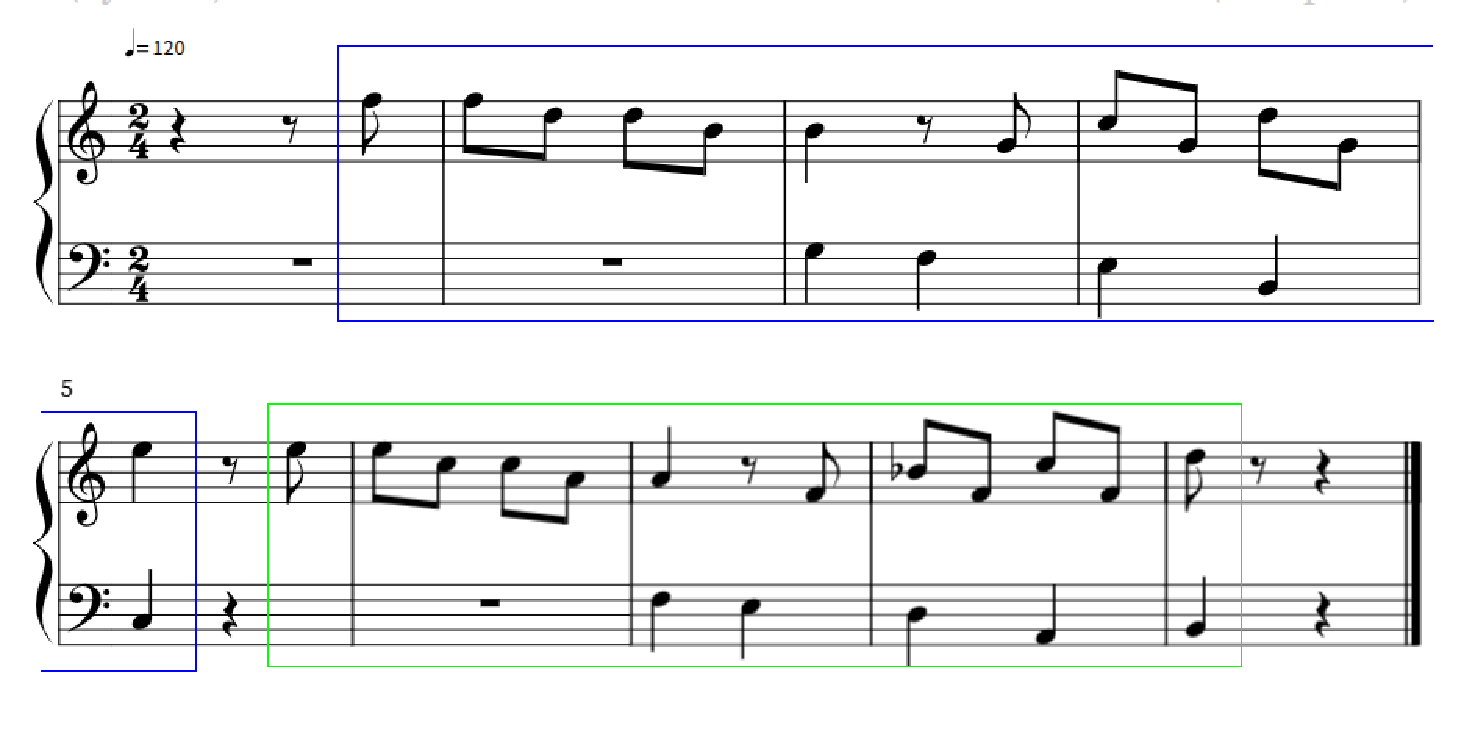
\includegraphics[scale=0.6]{obrazky-figures/motzartalegro.pdf}
    \caption{A small example of dependencies between music staffs.}
    \label{fig:sonatamultistring}
\end{figure}

Figure \ref{fig:sonatamultistring} comes from the development of \ref{fig:jazzclassic}. The second rectangle (green) is a variation of the notes selected in the first rectangle (blue). This can be easily encoded into the 2-component system
$$ G_s = (G_1, G_2, Q),$$ where

\begin{itemize}
    \item{$G_1 = (\{S_1, T, T_{\downarrow}\},\, \{f_{[-, e, 2]}, d_{[-, e, 2]}, h_{[-, e, 1]}, g_{[-, e, 1]}, c_{[-, e, 2]}, e_{[-, e, 2]}, 
    \\ r_{[-, q, -]}, r_{[-, e, -]}, f_{[\downarrow, e, 2]}, d_{[\downarrow, e, 2]}, h_{[\downarrow, e, 1]}, g_{[\downarrow, e, 1]}, c_{[\downarrow, e, 2]}, e_{[\downarrow, e, 2]}\},\, 
    \\ \{1: S_1 \rightarrow (T, T_{\downarrow}),  
    \\ 2: (T, T_{\downarrow}) \rightarrow (r_{[-, q, -]}r_{[-, e, -]}f_{[-, e, 2]}T, e_{[-, q, -]}r_{[-, e, -]}e_{[\downarrow, e, 2]}T_{\downarrow}), 
    \\ 3: (T, T_{\downarrow}) \rightarrow (f_{[-, e, 2]}, d_{[-, e, 2]}, d_{[-, e, 2]}, h_{[-, e, 1]}T, f_{[\downarrow, e, 2]}, d_{[\downarrow, e, 2]}, d_{[\downarrow, e, 2]}, h_{[\downarrow, e, 1]}T_{\downarrow}), 
    \\ 4: (T, T_{\downarrow}) \rightarrow (h_{[-, q, 1]}r_{[-, e, -]}g_{[-, e, 1]}T, h_{[\downarrow, q, 1]}, r_{[\downarrow, e, -]},  g_{[\downarrow, e, 1]}T_{\downarrow}),
    \\ 5: (T, T_{\downarrow}) \rightarrow (c_{[-, e, 2]}g_{[-, e, 1]}d_{[-, e, 2]}g_{[-, e, 1]}T, c_{[\downarrow, e, 2]}g_{[\downarrow, e, 1]}, d_{[\downarrow, e, 2]}g_{[\downarrow, e, 1]}T_{\downarrow}) 
    \\ 6: T_{\downarrow} \rightarrow (d_{[-, e, 2]}r_{[-, e, -]}r_{[-, q, -]})
    \})$,}
    \item{$G_2 = (\{S_2, B, B_{\downarrow}\},\, \{r_{[-, h, -]}, r_{[-, q, -]}, c_{[-, q, 2]}, g_{[-, q, 2]}, f_{[-, q, 2]}, g_{[\downarrow, q, 2]}, \\ f_{[\downarrow, q, 2]}, e_{[-, q, 2]}, h_{[-, q, 1]}, e_{[\downarrow, q, 2]}\}, \,
    \\\{1: S_2 \rightarrow (B, B_{\downarrow}), 
    \\ 2: (B, B_{\downarrow}) \rightarrow (r_{[-, h, -]}B, c_{[-, q, 2]}r_{[-, q, -]}B_{\downarrow}) 
    \\ 3: (B, B_{\downarrow}) \rightarrow (r_{[-, h, -]}B, r_{[-, h, -]}B_{\downarrow}), 
    \\ 4: (B, B_{\downarrow}) \rightarrow (g_{[-, q, 2]}f_{[-, q, 2]}B, g_{[\downarrow, q, 2]}f_{[\downarrow, q, 2]}B_{\downarrow}), 
    \\ 5: (B, B_{\downarrow}) \rightarrow (e_{[-, q, 2]}h_{[-, q, 1]}, e_{[\downarrow, q, 2]}h_{[\downarrow, q, 2]}B_{\downarrow}), 
    \\ 6: B_{\downarrow} \rightarrow (h_{[-, q, 1]}r_{[-, q, -]})\}$},
    \item{$Q = \{(1, 1), (2, 2), (3, 3), (4, 4), (5, 5), (6, 6)\}$.}
\end{itemize}

This shows how easy it is to encode one of the most popular classical songs into the grammar. Grammar $G_1$ has rules that can be applied to gererate the treble clef for piano and $G_2$ produces the bass clef. Each measure for both treble and bass clefs is synchronized in set $Q$.

\section{Derivation Process in Multi-Generative Grammar}
Derivation in formal language theory is a process in which the initial starting symbol is transformed or rewritten by rules until we reach the final string, which consists only of terminal symbols. A similar approach is used to generate music, with the key difference being that terminal symbols are interpreted as musical notes.

With the intention to create a music piece, rules have to be applied in a certain order. First, we rewrite starting symbol with nonterminals to define structure of the composition. With that, we can start to rewrite structure symbols so that final melodies and harmonies can take the form. 

To show this, let us start with an example that generates jazz music for two instruments: 
$$G_s = (G_1, G_2, Q),$$ in which 
\begin{itemize}
    \item{$G_1 = (\{S_1, A, B\},\, \{c_{y}, a_{x}, g_{x}, e_{y},f_{x},\alpha_{z},\beta_{z},\gamma_{z},\delta_{z},\epsilon_{w},\zeta_{w}\},\, 
    \\ \{1: S_1 \rightarrow (AABAS_1),
    \\ 2: S_1 \rightarrow (AABA),
    \\ 3: (A, A, A) \rightarrow (MH, MH, MH), 
    \\ 4: (M, M, M) \rightarrow (c_{y}c_{y}a_{x}g_{x}, c_{y}c_{y}a_{x}g_{x}, c_{y}c_{y}a_{x}g_{x}),
    \\ 5: (H, H, H) \rightarrow (\alpha_{z}\beta_{z}\gamma_{z}\delta_{z}, \alpha_{z}\beta_{z}\gamma_{z}\delta_{z}, \alpha_{z}\beta_{z}\gamma_{z}\delta_{z}),
    \\ 6: (B) \rightarrow (H_1M_1),
    \\ 7: (H_1, M_1) \rightarrow (\epsilon_{w}\zeta_{w}, e_{y}a_{x}f_{x}a_{x})
    \})$,}
    \item{$G_2 = (\{S_2, A, B, P, L\},\, \{c_{v}, g_{v}, r_{v}, a_{u}, e_{v}, r_{t}\}, \,
    \\\{1: S_2 \rightarrow (AABAS_2),
    \\ 2: S_2 \rightarrow (AABA),
    \\ 3: (A, A, A) \rightarrow (PL, PL, PL), 
    \\ 4: (P, P, P) \rightarrow (c_{v}g_{v}c_{v}g_{v}r_{v}g_{v}c_{v}g_{v}, c_{v}g_{v}c_{v}g_{v}r_{v}g_{v}c_{v}g_{v}, c_{v}g_{v}c_{v}g_{v}r_{v}g_{v}c_{v}g_{v}),
    \\ 5: (L, L, L) \rightarrow (c_{v}a_{u}e_{s}r_{v}r_{t}e_{s}a_{u}, c_{v}a_{u}e_{s}r_{v}r_{t}e_{s}a_{u}, c_{v}a_{u}e_{s}r_{v}r_{t}e_{s}a_{u}),
    \\ 6: (B) \rightarrow (PL),
    \\ 7: (P, L) \rightarrow (c_{v}g_{v}c_{v}g_{v}r_{v}g_{v}c_{v}g_{v}, c_{v}a_{u}e_{s}r_{v}r_{t}e_{s}a_{u})
    \})$,}
    \item{$Q = \{(1, 1), (2, 2), (3, 3), (4, 4), (5, 5), (6, 6), (7, 7)\}$.}
\end{itemize}

Grammars in system $G_{s}$ use substitution of token symbols for better readability in~defined grammar and in~following derivations. Explanation of the tokens in grammar $G_1$ is in the table \ref{Tb1} and for $G_2$ in $\ref{Tb2}$. The defined system has extra substitution for the token attributes in comparison to the following examples in other sections. This was done to make derivation steps more readable.
\begin{table}[h]
\centering
\begin{minipage}{0.48\textwidth}
\centering
\begin{tabular}{c|c}
Symbol & Note and Chord \\
\hline
$c_y$ & $c_{[-, q, 2]}$ \\
$a_x$ & $a_{[-, q, 1]}$ \\
$g_x$ & $g_{[-, q, 1]}$ \\
$e_y$ & $e_{[-, q, 2]}$ \\
$f_x$ & $f_{[-, q, 1]}$ \\
$\alpha_{z}$ & $Chord(C,C,E)_{[-, q, 1]}$ \\
$\beta_{z}$ & $Chord(D,F,A)_{[-, q, 1]}$ \\
$\gamma_{z}$ & $Chord(A,C,F)_{[-, q, 1]}$ \\
$\delta_{z}$ & $Chord(A,C,E)_{[-, q, 1]}$ \\
$\epsilon_{w}$ & $Chord(A,C,F)_{[-, h, 1]}$ \\
$\zeta_{w}$ & $Chord(F,A,C)_{[-, h, 1]}$ \\
\end{tabular}
\caption{Mapping of terminal symbols to their note interpretation for $G_1$.}
\label{Tb1}
\end{minipage}
\hfill
\begin{minipage}{0.48\textwidth}
\centering
\begin{tabular}{c|c}
Symbol & Note and Chord \\
\hline
$c_{v}$ & $c_{[-, e, 1]}$ \\
$g_{v}$ & $g_{[-, e, 1]}$ \\
$r_{t}$ & $r_{[-, e, 1]}$ \\
$a_{u}$ & $a_{[\flat, e, 1]}$ \\
$e_{v}$ & $e_{[\flat, e, 1]}$ \\
$r_{t}$ & $r_{[-, e, 1]}$ \\
\end{tabular}
\caption{Mapping of terminal symbols to their note interpretation for $G_2$.}
\label{Tb2}
\end{minipage}
\end{table}

For this $G_s$, we can create the following derivation steps:
\begin{itemize}
    \item{$(S_1, S_2) \Rightarrow^1 (AABA, AABA) \Rightarrow^2 (HMHBMH, PLPLBPL) 
    \\ \Rightarrow^3 (c_{y}c_{y}a_{x}g_{x}Hc_{y}c_{y}a_{x}g_{x}HM_1H_1c_{y}c_{y}a_{x}g_{x}H, 
    \\ c_{v}g_{v}c_{v}g_{v}r_{v}g_{v}c_{v}g_{v}Lc_{v}g_{v}c_{v}g_{v}r_{v}g_{v}c_{v}g_{v}LPLc_{v}g_{v}c_{v}g_{v}r_{v}g_{v}c_{v}g_{v}L)
    \\ \Rightarrow \hdots$}
\end{itemize}

Instead of writing out terminal symbols, it is much more interesting to demonstrate terminal symbols already in the music staff. Nonterminal symbols are blank bars that represent the structure. Fig.~\ref{fig:def1final1} describes the correspondence between the third and fourth derivation steps in $G_s$ and their musical interpretation. More specifically, during $\Rightarrow^3$, $G_s$ rewrites nonterminals $H$ and $L$ from $G_1$ and $G_2$, respectively; as a result, all A parts are completed.  During $\Rightarrow^4$, $G_s$ completes the generation of the sentence and, therefore, its corresponding musical piece by filling in the missing part of the generated score.

\begin{figure}[H]
\centering
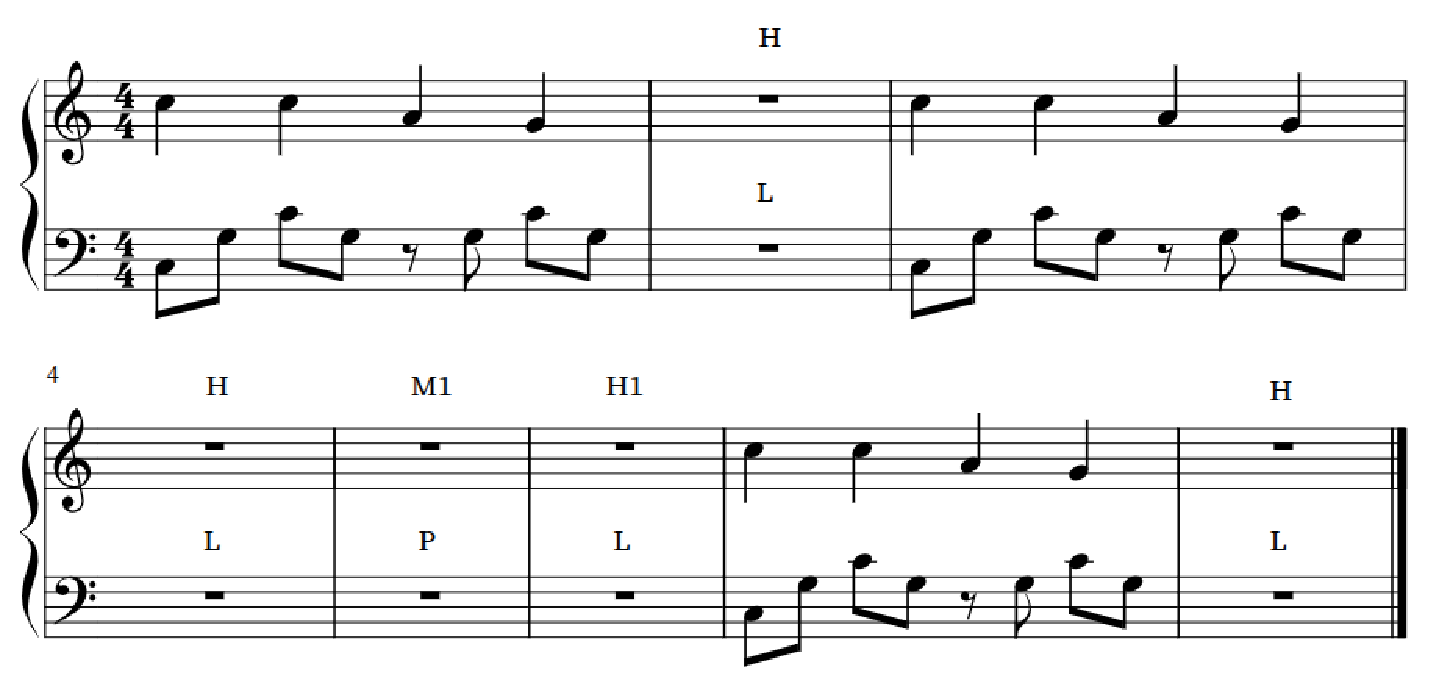
\includegraphics[scale=0.35]{obrazky-figures/der3.pdf}
\[
\Rightarrow^3
\]
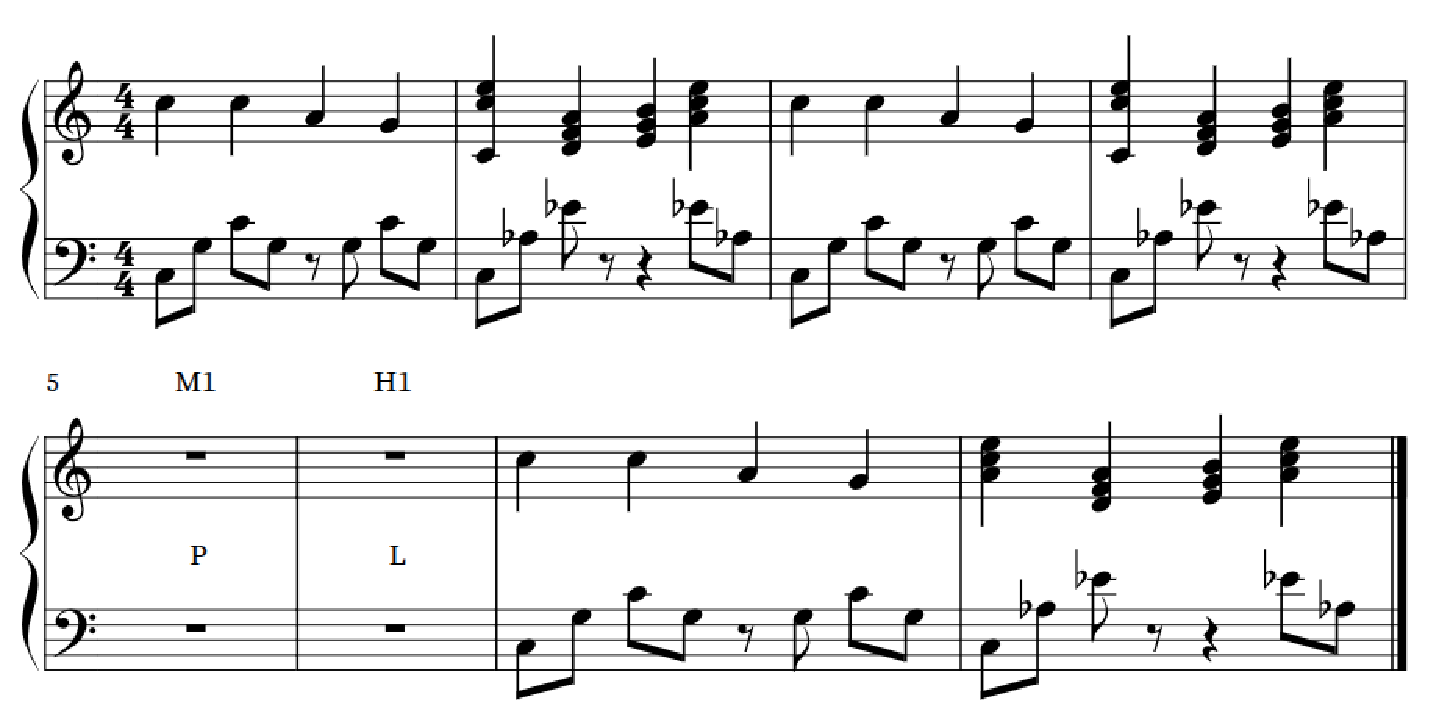
\includegraphics[scale=0.35]{obrazky-figures/der4.pdf}
\[
\Rightarrow^4
\]
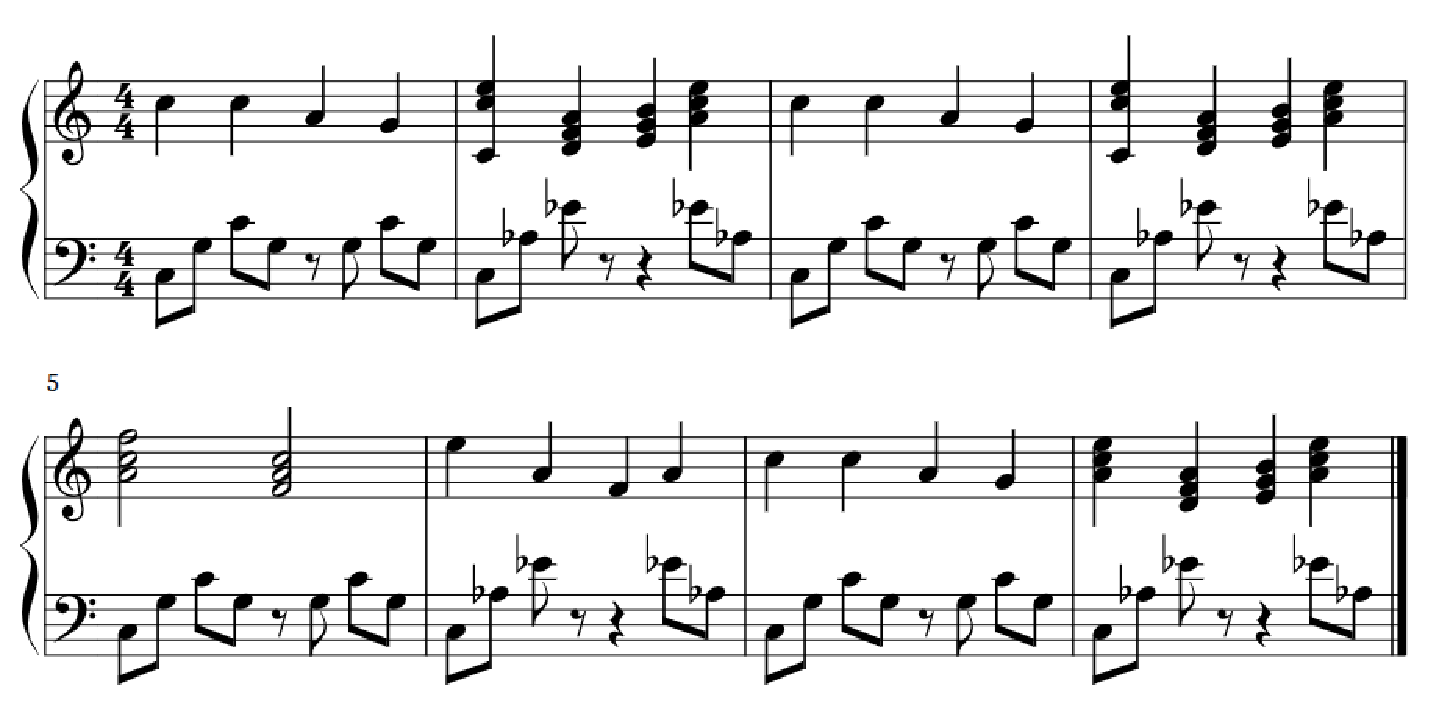
\includegraphics[scale=0.35]{obrazky-figures/der5.pdf}
\caption{The third and fourth derivation step shown in music staff that corresponds to $(5,5) \in Q$, and $(7,7) \in Q$.}
\label{fig:def1final1}
\end{figure}

To give a better explanation of what our grammar generates. It is a jazz piano solo in the mentioned form. The bass clef is there to provide background for the main theme, which is generated in the treble clef. What we used for it is a simple PL cycle. The treble clef contains A part that consists of one melody and one harmonic part. Similarly, in~contrast, section B starts with the harmonic part from chords and ends with a melody that is connected to the last repetition of the main theme.

\section{Algorithmic Implementation of the Model}
\label{sec:algimp}
As it is in all aspects of informatics to make our model work in a program, there is a need for an algorithm that makes it run. Because of that, we have formed a simple algorithm that generates multi-string and is presented in Algorithm \ref{alg:multistring}.

As an input, the algorithm takes grammar system $G_s$. This system has to contain scattered context grammars that have rules for structure and tokens. The application of rules defined in each grammar is non-deterministic. Because of this, the implementation must determine which rule to apply by making a random choice. Defined grammars could have endless possibilities for rules that could be applied. To avoid that, we also put the number of repetitions as an input argument. This number determines how many times a specific rule with a nonterminal on the right-hand side can be applied in a row. For example a rule $(A, A) \Rightarrow (TH, TH)$ can be applied maximum of \textit{repetition} times. This ensures that at some point, all nonterminals will be rewritten using tone rules and limits tedious repetitions that happen with too many similar structural parts. This parameter was inspired by the iterative parameter used in L-systems.

The algorithm begins by initializing the multi-string with starting symbol for each grammar. Next, the list of applied rules is initialized. We want to keep the list of rules that are applied during the derivation process for composer.

For didactic reasons, we have decided to split the algorithm into two parts. The first part identifies and applies structure rules, while the second loop applies rules that generate final tokens, which are then interpreted as musical output. The union of structure rules and token rules constitutes the complete rule set for each component of the grammar system.

After that, we enter the nested \textit{while} loop that controls the number of repetitions. Inside this loop, we select a component from the grammar system. Before performing a derivation step, we retrieve the current string for this component along with the list of rules that have already been applied. We search for nonterminals that can be rewritten using structure rules in this string. If a rule is applicable, it is selected and applied. Then, we retrieve a~tuple of corresponding rules for the other components to maintain synchronization. This can be handled in multiple ways; in our case, we keep these tuples indexed by the rule applied in the selected component.

Synchronization is performed in the nested \textit{forall} loop, where the corresponding rules are applied to all components, and their derivation steps are stored. This process is repeated for every nonterminal generated from the start symbol at least once and continues until the repetition limit is reached. Once the limit is met, rewriting stops. In the case of structure rules, the algorithm moves on to tone rules; in the case of tone rules, the algorithm terminates and returns the resulting multi-string along with the list of derivation steps.

The repetition counter $i$ is incremented only after all nonterminals have been rewritten at least once.

\begin{algorithm}[H]
\DontPrintSemicolon
\SetAlgoLined
\KwIn{Grammar system $G_s$, repetitions}
\KwOut{Multi-string $M$}

Initialize $M$ using start symbols of each instrument\;
Set steps for each instrument $\gets [\,]$\;

\ForEach{rule type $\in \{\text{structure}, \text{tone}\}$}{
    Set $i \gets 0$\;

    \While{$i \leq$ repetitions}{
        \ForEach{$G_c \in G_s$}{
            $current \gets M[G_c]$\;
            $steps \gets steps[G_c]$\;

            \If{$r_c: (A_1,\dots,A_n) \rightarrow (x_1,\dots,x_n)$ of the given type is applicable to $current$}{
                \If{$i = repetitions$}{
                    $r_c: \ (A_1,\dots,A_k) \rightarrow (\alpha_1,\dots,\alpha_k)\ \text{has only terminals if}\ \forall i,\ \alpha_i \in T^*$
                }

                Retrieve synchronization tuple $q = Q[r_c]$\;

                \ForAll{$G_j \in G_s$}{
                    $r_j \gets q[G_j]$\;
                    \If{$r_j$ is applicable to $M[G_j]$}{
                        Apply rule $r_j$ to $M[G_j]$\;
                        Append $r_j$ to $steps[G_j]$\;
                    }
                }
            }
        }

        Increment $i$\;
    }
}

\Return{$M$, steps}
\caption{Generate Multi-string Music from Grammar System}
\label{alg:multistring}
\end{algorithm}

\section{Examples of Generated Music}
We have already shown some fascinating examples from classical and jazz music. To show how capable our model truly is and that it can generate all kinds of incredible melodies and harmonies, not just fractal-like ones or things tied to a specific genre, we have dedicated this section to that purpose. In the following examples, we skip writing out the terminal symbols and create a convention that each lowercase letter in a rule is a terminal symbol.

\subsection*{Single Instrument}
This time, to demonstrate the capabilities of the model and what it can generate, We have prepared a guitar solo with a custom form. In this case, the model reduces to a scattered context grammar, but it still preserves all the core musical characteristics. We have decided to shape the music with a clear form, built around two main ideas that are worth to explore. Sometimes, musicians use interesting transitions to connect ideas, and we aim to use one to make the second theme more musically appealing. 

The first main idea will be built on top of the melodic and harmonic parts and will end a song with their variations. The second idea should be mirrored and contain a small transition. For that, we have designed a grammar that would look like this:

$$G_s = (G_1, Q),$$ in which 
\begin{itemize}
    \item{$G_1 = (\{S, A, B, C, M, H, M_1, H_1\},\,\, 
    \\ \{1: S \rightarrow (ABCB^{R}A),
    \\ 2: (A, A) \rightarrow (MMHH, MMHH), 
    \\ 3: (B,B^{R}) \rightarrow (M_1H_1, H_1M_1),
    \\ 4: (C)  \rightarrow (\alpha_{[-, q, 1]},\beta_{[-, h, 1]},\alpha_{[-, q, 1]}),
    \\ 5: (M, M)  \rightarrow (g_{[-, q, 1]}a_{[-, q, 1]}g_{[-, q, 1]}e_{[-, q, 1]}M, g_{[\gg, q, 1]}a_{[\gg, q, 1]}g_{[\gg, q, 1]}e_{[\gg, q, 1]}M),
    \\ 6: (M, M)  \rightarrow (g_{[-, q, 1]}g_{[-, q, 1]}a_{[-, q, 1]}c_{[-, q, 2]}M, g_{[\gg, q, 1]}g_{[\gg, q, 1]}a_{[\gg, q, 1]}c_{[\gg, q, 2]}M),
    \\ 7: (M_1, M_1)  \rightarrow (g_{[-, q, 1]}g_{[-, q, 1]}e_{[-, q, 1]}e_{[-, q, 1]}, g_{[\bowtie, q, 1]}g_{[\bowtie, q, 1]}e_{[\bowtie, q, 1]}e_{[\bowtie, q, 1]}),
    \\ 8: (H, H)  \rightarrow (\delta_{[-, q, 1]}\theta_{[-, q, 1]}\beta_{[-, q, 1]}\eta_{[-, q, 1]}H, \delta_{[-, q, 1]}\theta_{[-, q, 1]}\zeta_{[-, q, 1]}\eta_{[-, q, 1]}H),
    \\ 9: (H, H)  \rightarrow (\delta_{[L, q, 1]}\theta_{[L, q, 1]}\beta_{[L, q, 1]}\eta_{[L, q, 1]}H, \delta_{[L, q, 1]}\theta_{[L, q, 1]}\zeta_{[L, q, 1]}\eta_{[L, q, 1]}H),
    \\ 10: (H_1, H_1)  \rightarrow (\beta_{[-, q, 1]}\eta_{[-, q, 1]}\delta_{[-, q, 1]}\theta_{[-, q, 1]}, \beta_{[\uparrow, q, 1]}\eta_{[\uparrow, q, 1]}\delta_{[\uparrow, q, 1]}\theta_{[\uparrow, q, 1]}),
    \\ 11: (M, M)  \rightarrow (\epsilon, \epsilon),
    \\ 12: (H, H)  \rightarrow (\epsilon, \epsilon)
    \})$,}
    \item{$Q = \{\}$.}
\end{itemize}

\begin{table}[h]
\centering
\begin{tabular}{c|c}
Symbol & Chord \\
\hline
$\alpha$ & $Chord(E,G,H)$ \\
$\beta$ & $Chord(A,C,E)$ \\
$\delta$ & $Chord(C,E,G)$ \\
$\theta$ & $Chord(G,H,D)$ \\
$\eta$ & $Chord(F,A,C)$ \\
\end{tabular}
\label{Tb3}
\caption{Mapping of terminal symbols to musical chords for $G_1$.}
\end{table}

The grammar contains two new operations that are being applied to tones from the measure on the left side. The first operation is $\gg$ which denotes chromatic shift by major third inspired by \cite{kim2007liszt}. The second operation is counterpoint, denoted by 
$\bowtie$, which we adopt from \cite{yearsley2002bach}, as this technique was popularized by J. S. Bach. It takes the first note and shifts it up by an interval of 3, the second note by 4, the third by 6, and then this pattern is repeated for the following notes. The well-known $\uparrow$ just moves all notes in the measure up by one whole tone.

Let us start generating guitar solos. For this $G_s$, we can create the following derivation steps:
\begin{itemize}
    \item{$S_1 \Rightarrow^1 ABCB^{R}A \Rightarrow^2 MMHHBCB^{R}MMHH \Rightarrow^3 MMHHM_1H_1CH_1M_1MMHH
    \\ \Rightarrow \hdots$}
\end{itemize}

In the following derivation steps, all $M$ and $H$ nonterminals will be replaced with terminal symbols (notes) using rules 5, 6, 7, and 8. Following interpretation in music staff is shown in Figure \ref{fig:def1final2}. The upper part of the image displays rewritten all $M$ and $H$ nonterminals. The middle part represents two derivation steps $\Rightarrow^8$ and $\Rightarrow^9$ where nonterminals $M_1$ and $H_1$ are rewritten. And the last derivation step $\Rightarrow^{10}$ replaces nonterminal $C$ to form the final music piece.

\begin{figure}[H]
\centering
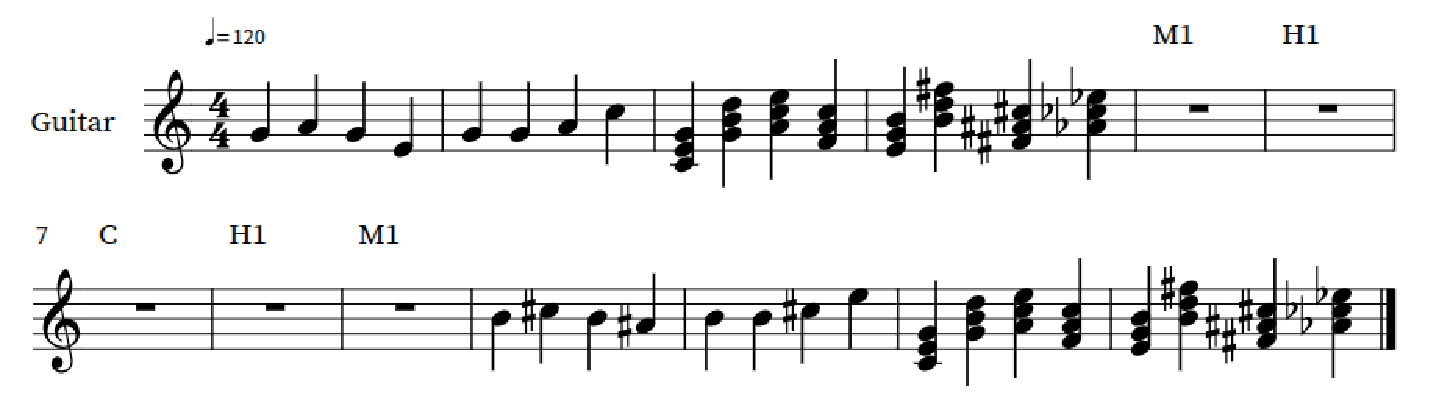
\includegraphics[scale=0.35]{obrazky-figures/Ste1.pdf}
\[
\Rightarrow^8 ... \Rightarrow^9
\]
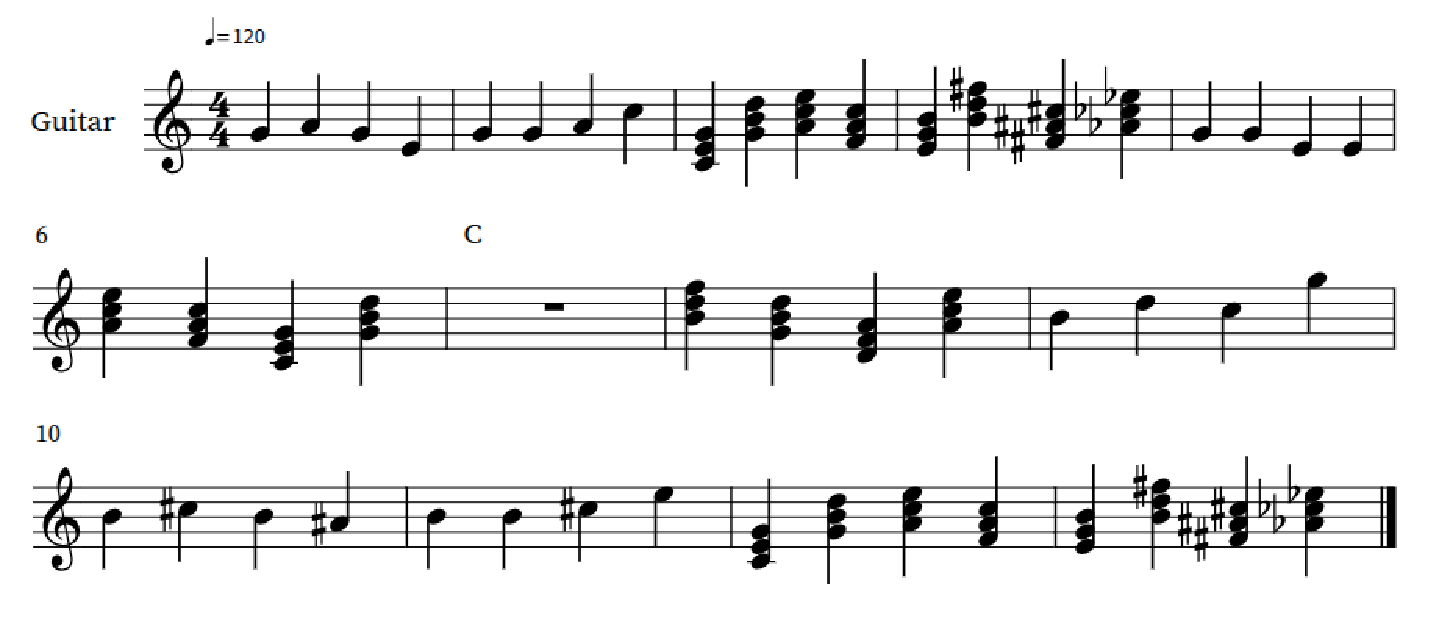
\includegraphics[scale=0.35]{obrazky-figures/Ste2.pdf}
\[
\Rightarrow^{10}
\]
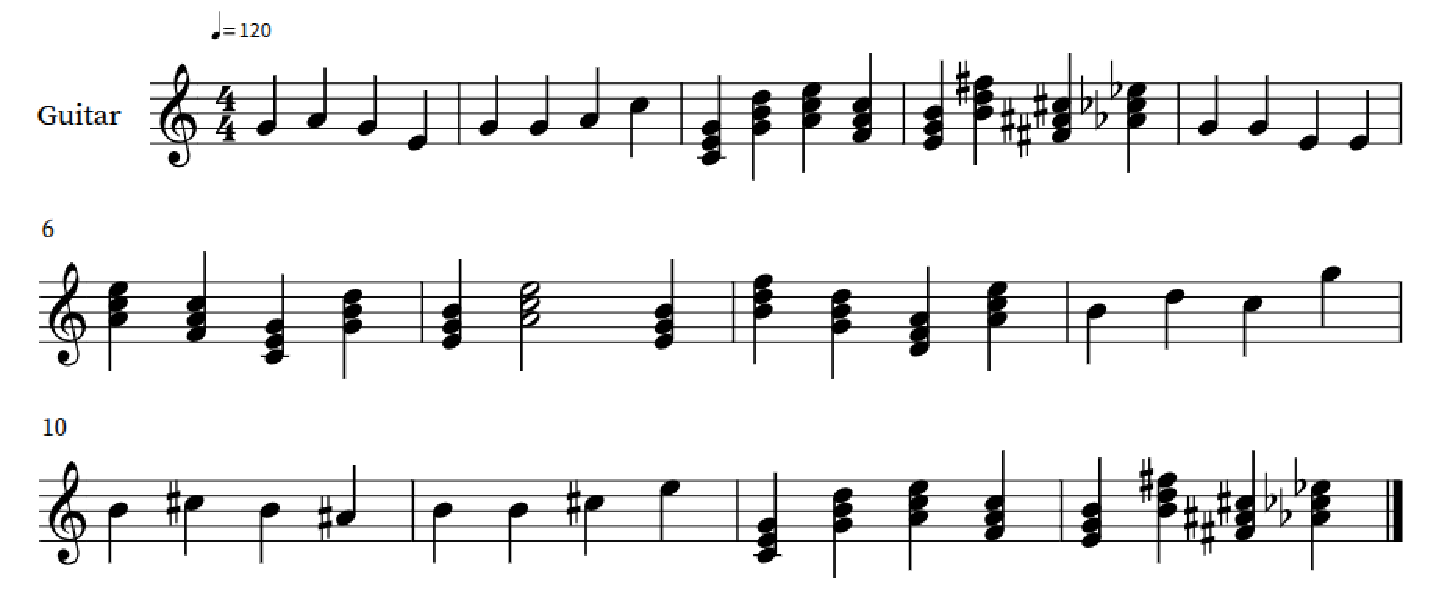
\includegraphics[scale=0.35]{obrazky-figures/Ste3.pdf}
\caption{Interpretation of derivation steps in music staff.}
\label{fig:def1final2}
\end{figure}

\subsection*{Multiple Instruments}
Until now, we have been generating music for only one instrument. Finally, we will show how our model could generate jazz music. This music is going to be interpreted by a~piano and a~saxophone. The music will take jazz from AABA and will be generated in three strings, two for piano and one for saxophone. So far, we have used variation, tone duration, and tone octave for our generated tokens. Now, we will also incorporate dynamics. An~example of grammar system generating such computation follows

$$G_s = (G_1, G_2, G_3, Q),$$ in which 
\begin{itemize}
    \item{$G_1 = (\{S_1, M_1, M_2, A, B, N\},\,\, 
    \\ \{1: S \rightarrow (AAABA),
    \\ 2: (A, A, A) \rightarrow (M_1M_2M_2M_1, M_1M_2M_2M_1, M_1M_2M_2M_1),
    \\ 3: (M_1, M_1, M_1) \rightarrow (f_{[-, q, 1, -]}c_{[-, q, 1, -]}c_{[-, h, 1, -]}, 
    \\f_{[\downarrow, q, 1, p]}c_{[\downarrow, q, 1, p]}c_{[\downarrow, h, 1, p]}, f_{[-, q, 1, -]}c_{[-, q, 1, -]}c_{[-, h, 2, -]}),
    \\ 4: (M_1, M_1, M_1) \rightarrow (g_{[-, q, 2, -]}d_{[-, q, 2, -]}d_{[-, h, 2, -]}, 
    \\g_{[\downarrow, q, 2, p]}d_{[\downarrow, q, 2, p]}d_{[\downarrow, h, 2, p]}, g_{[-, q, 2, -]}d_{[-, q, 2, -]}d_{[-, h, 2, -]}),
    \\ 5: (M_2, M_2, M_2) \rightarrow (e_{[-, h, 2, -]}g_{[-, h, 2, -]}, e_{[\downarrow, h, 2, p]}g_{[\downarrow, h, 2, p]}, e_{[-, h, 2, -]}g_{[-, h, 2, -]}),
    \\ 6: (M_2, M_2, M_2) \rightarrow (f_{[-, h, 2, -]}a_{[-, h, 2, -]}, f_{[\downarrow, h, 2, p]}a_{[\downarrow, h, 2, p]}, f_{[-, h, 2, -]}a_{[-, h, 2, -]}),
    \\ 7: B \rightarrow (NNNN)
    \\ 8: N \rightarrow (r_{[-, f, -, -]})
    \})$,}
    \item{$G_2 = (\{S_2, A, B, P, R, N\},\, \, 
    \\ \{1: S \rightarrow (AAABA),
    \\ 2: (A, A, A) \rightarrow (PRPR, PRPR, PRPR), 
    \\ 3: (P, P, P) \rightarrow (\gamma_{[-, h, 1, -]}\gamma_{[P, h, 1, -]}R, \gamma_{[-, h, 1, p]}\gamma_{[P, h, 1, p]}R, \gamma_{[-, h, 1, -]}\gamma_{[P, h, 1, -]}R),
    \\ 4: (R, R, R) \rightarrow (\gamma_{[-, h, 1, -]}\gamma_{[R, h, 1, -]}P, \gamma_{[-, h, 1, p]}\gamma_{[R, h, 1, p]}P, \gamma_{[-, h, 1, -]}\gamma_{[R, h, 1, -]}P),
    \\ 5: (P, P, P) \rightarrow (\gamma_{[-, h, 1, -]}\gamma_{[P, h, 1, -]}, \gamma_{[-, h, 1, p]}\gamma_{[P, h, 1, p]}, \gamma_{[-, h, 1, -]}\gamma_{[P, h, 1, -]}),
    \\ 6: (R, R, R) \rightarrow (\gamma_{[-, h, 1, -]}\gamma_{[R, h, 1, -]}, \gamma_{[-, h, 1, p]}\gamma_{[R, h, 1, p]}, \gamma_{[-, h, 1, -]}\gamma_{[R, h, 1, -]}),
    \\ 7: B \rightarrow (NNNN)
    \\ 8: N \rightarrow (r_{[-, f, -, -]})
    \})$,}
    \item{$G_3 = (\{S_3, A, B, H, M_{31}, M_{32}\},\, \, 
    \\ \{1: S \rightarrow (AAABA),
    \\ 2: (A, A, A) \rightarrow (MMMM, MMMM, MMMM),
    \\ 3: (M, M, M) \rightarrow (e_{[-, h, 1, -]}g_{[-, h, 1, -]}, e_{[\uparrow, h, 1, -]}g_{[\uparrow, h, 1, -]}, e_{[-, h, 1, -]}g_{[-, h, 1, -]}),
    \\ 4: (M, M, M) \rightarrow (a_{[-, h, 1, -]}f_{[-, h, 1, -]}, a_{[\uparrow, h, 1, -]}f_{[\uparrow, h, 1, -]}, a_{[-, h, 1, -]}f_{[-, h, 1, -]}),
    \\ 5: (M, M, M) \rightarrow (g_{[-, h, 1, -]}e_{[-, h, 1, -]}, g_{[\uparrow, h, 1, -]}e_{[\uparrow, h, 1, -]}, g_{[-, h, 1, -]}e_{[-, h, 1, -]}),
    \\ 6: (M, M, M) \rightarrow (f_{[-, h, 1, -]}f_{[-, h, 1, -]}, f_{[\uparrow, h, 1, -]}f_{[\uparrow, h, 1, -]}, f_{[-, h, 1, -]}f_{[-, h, 1, -]}),
    \\ 7: B \rightarrow (HM_{31}M_{32}H)
    \\ 8: (H, H) \rightarrow (\alpha_{[-, h, 1, -]}\beta_{[-, h, 1, -]}, \alpha_{[r, h, 1, -]}\beta_{[r, h, 1, -]})
    \\ 9: M_{31} \rightarrow (e_{[-, h, 1, -]}g_{[-, h, 1, -]}a_{[-, h, 1, -]}h_{[-, h, 1, -]})
    \\ 10: M_{32} \rightarrow (h_{[-, q, 1, -]}c_{[-, q, 1, -]}a_{[-, q, 1, -]}f_{[-, q, 1, -]})
    \})$,}
    \item{$Q = \{(1, 1, 1), (2, 2, 2), (3, 3, 3), (3, 5, 3), (4, 4, 4), (4, 6, 4), (5, 4, 5), (5, 6, 5), \\ (6, 3, 6), (6, 5, 6), (7, 7, 7), (8, 8, 8), (8, 8, 9), (8, 8, 10)\}$.}
\end{itemize}

The Greek alphabet terminals are chords and they would be interpreted according to these tables:

\begin{table}[h]
\centering
\begin{minipage}{0.48\textwidth}
\centering
\begin{tabular}{c|c}
Symbol & Note \\
\hline
$\gamma$ & $Chord(C,E,G)$ \\
$\gamma$ & $Chord(C,Es,G)$ \\
$\gamma$ & $Chord(Es,G,Ces)$ \\
$\gamma$ & $Chord(Es,Ges,Ces)$ \\
$\gamma$ & $Chord(Ges,Hes,Des)$ \\
\end{tabular}
\caption{Mapping of terminal symbols to chords from the Tonnetz walk using PR transformations of $G_2$.}
\label{Tb4}
\end{minipage}
\hfill
\begin{minipage}{0.48\textwidth}
\centering
\begin{tabular}{c|c}
Symbol & Chord \\
\hline
$\alpha$ & $Chord(A,C,E)$ \\
$\beta$ & $Chord(E,G,H)$ \\
\end{tabular}
\caption{Mapping of terminal symbols to music chords for $G_3$.}
\label{Tb5}
\end{minipage}
\end{table}

A composition that could be generated by the presented grammar system is shown in the Figure \ref{fig:JazzExamples}. It shows that grammar can generate meaningful music with various music techniques. To describe what is in the figure, we would start with the piano part. In the piano part, the $A$ (nonterminal in rule) interpreted as section of the composition presents the main theme and completes the harmony in the treble clef, while additional harmonic support is found in the bass clef. Alongside the piano, the saxophone is there to provide a second harmonic party to enrich the melody. The role of the saxophone is to create an~interesting contrast to the main melody. While the primary theme ascends, the saxophone line moves downwards, creating playful tension and enriching the overall texture. A bridge ($B$) is created by saxophone solo, which is an alternation between harmonic and melodic material to create contrast with the $A$ sections and a bridge between the piano part of the main theme and the last repetition of the main theme that ends the composition. 
\begin{figure}[H]
\centering
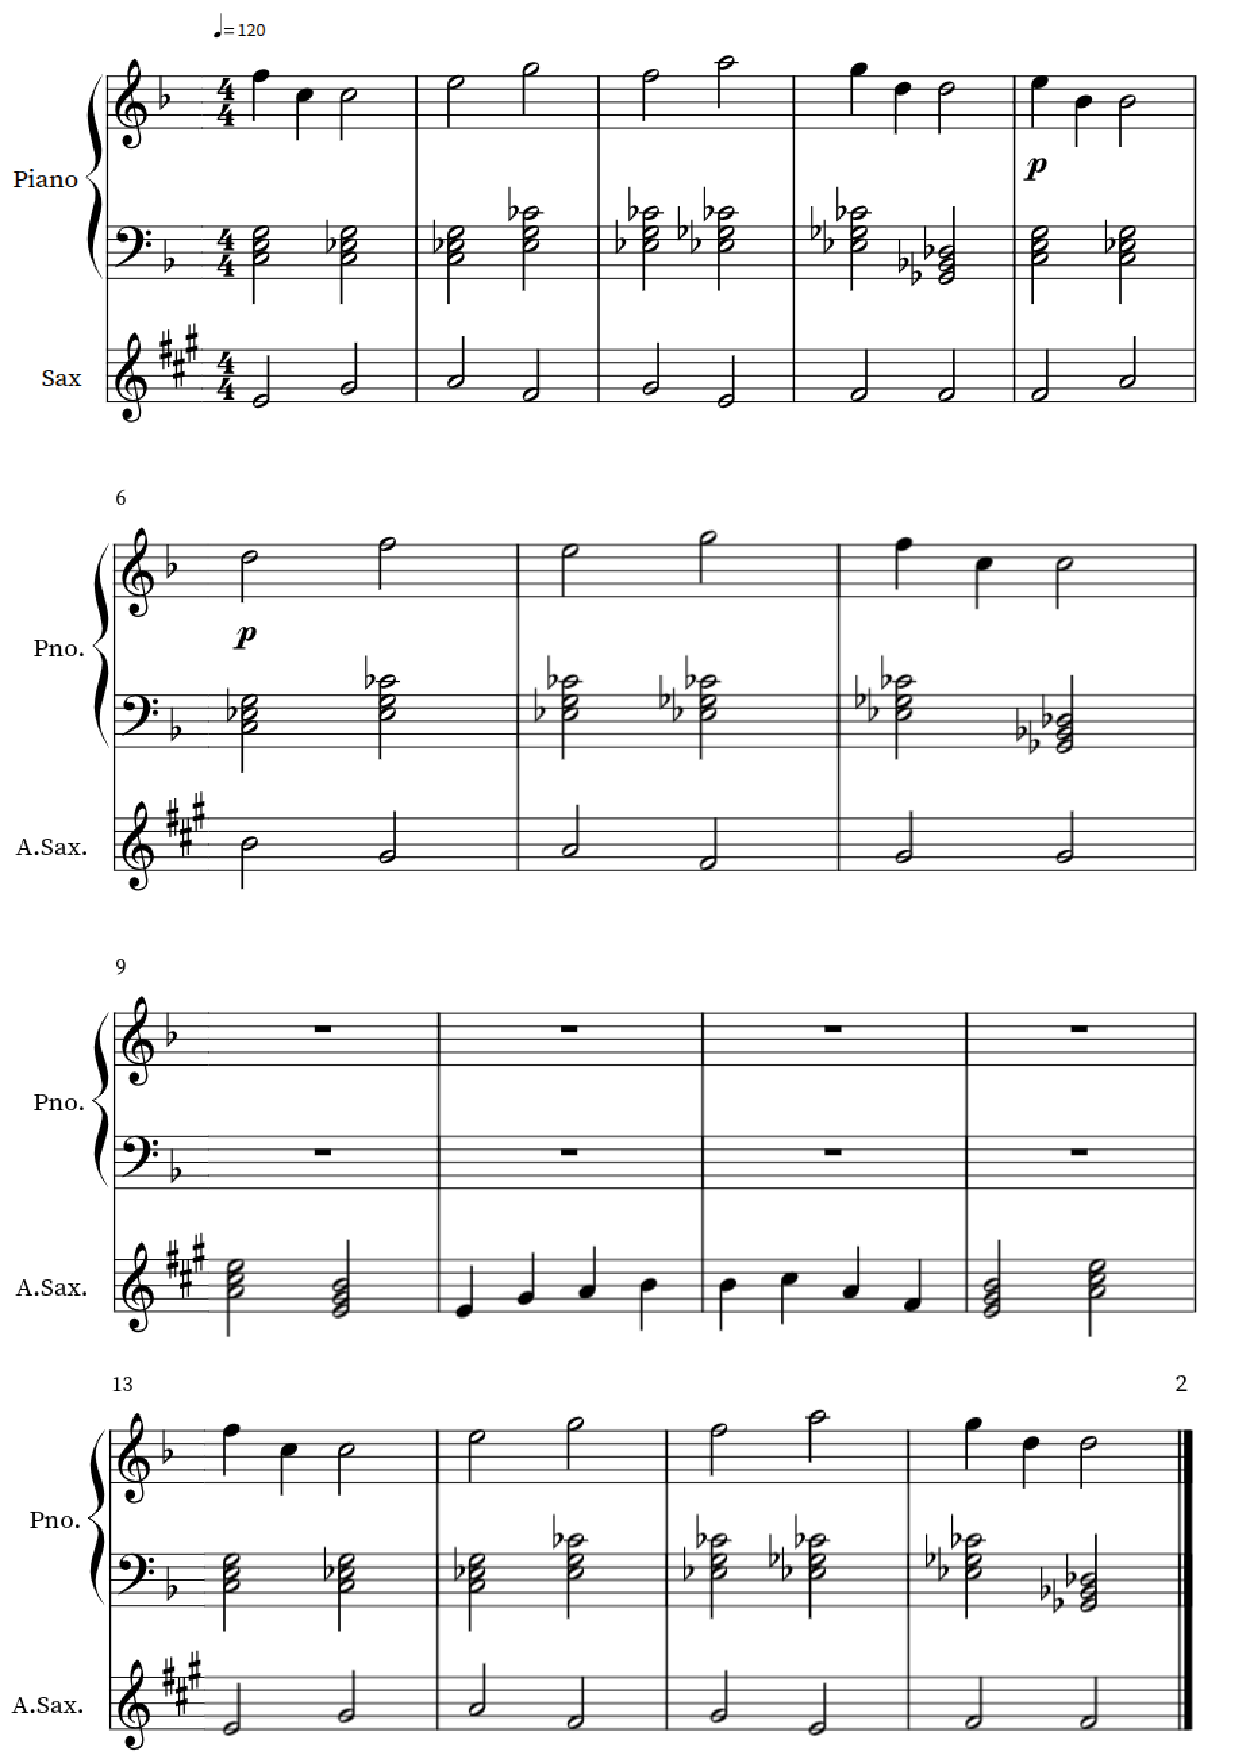
\includegraphics[scale=0.5]{obrazky-figures/Example-Jazz/Fullmusicexample.pdf}
\caption{Illustrative example of multi-instrument jazz composition.}
\label{fig:JazzExamples}
\end{figure}
Another example with 4 components could be found in the Appendix \ref{app:example}.

\subsection*{Constraints and Limitations}
The presented model applies transformation rules in a non-deterministic manner. Although rule selection is random, it will require external guidance from the software or human who designs the rules. Another factor is determining the correct synchronization states and coordinated rule application across all instruments. Because of that, the model can not live by itself, and it needs a composer or framework that will generate rules for it. A limitation could be that everything about the music must be defined. Each instrument needs to have defined rules, and all instruments must participate in the synchronization steps. 

As with most symbolic models, this system treats music as a sequence of abstract symbols, which means it inherently lacks a deep musical understanding. The quality of the output is tied to the design of the rule system. The model itself does not possess musical intuition. We attempted to build in structures for melody, harmonic progression, dynamics, and style, but while some musical dimensions can be encoded, others remain difficult or impractical to model quality.

This model can face issues with scalability. The amount of music this model creates is restricted to the amount of rules provided by specific system components. With a large number of rules, the complexity of the model increases. This can cause a decline in music quality and make the model difficult to manage, debug, or optimize.

The system is not designed to generate long-form music, such as multi-hour compositions or large soundtracks. Instead, its use case is to produce short, musically interesting sequences like melodies, harmonies, and textures lasting a few minutes. This limited scope is not a weakness, but rather the sweet spot of the model for which it was intended.

\chapter{Implementation}
\label{chap5}
The theory in previous sections would not mean much without a proper demonstration in~practice. We have decided to develop a console application in a similar way as in~\cite{eibensteiner2018procedural}. Console application presented in this chapter implements algorithm Alg.~\ref{alg:multistring}. It takes a~JSON file containing the grammar system definition as input and produces a MIDI file as output. 
The output file can then be played or used as an input file for other programs or components.

\section{Used Technologies}
The implementation was done in the Python programming language and uses standard and external libraries. Those libraries are listed in the readme file, and the most important one is discussed in this section. 

Many cited works use for music generation MIDI standard. As discussed in \cite{muller_midi}, it is considered to be stable in the music industry, and with its help, the musician can manipulate and work with multiple instruments in real time. This standard is popular and used in applications up to this date. MIDI file contains MIDI messages. The most important MIDI messages are note off and note on commands. With them we can define start and end of a note. These commands can include attributes that define pitch, velocity, channel, and time. Pitch is self-explanatory; velocity determines the dynamics, the channel specifies the instrument for the note, and time indicates the number of ticks to wait before the next message. To work with MIDI in Python we have used mido library \cite{mido}.

\section{Inputs and Outputs}
The application reads the input file in JSON format, which contains the full definition of the grammar system. This format is commonly used in Python applications, and it corresponds to a Python dictionary that helps with efficient manipulation. 

A full example is not listed here because of its length, but one can be found in an Appendix \ref{app:content}, and other interesting examples are stored in a source folder with the application. Instead of including the entire input file in this text, we have decided to give a step-by-step explanation of the components and attributes that are stored in the file.

Top level key \texttt{instruments} is a dictionary that stores components of multigenerative grammar systems. Each component corresponds to an instrument and is identified directly by its name.

\begin{verbatim}
"instruments": {
    "Piano_treble": { ... },
    "Piano_bass": { ... }
}
\end{verbatim}

Each instrument stores information as a grammar nonterminal, terminal, and starting symbol. To simplify implementation, we have decided to store structure rules and tone rules in different lists. This is because nonterminals do not store as many attributes as tone rules.

\begin{itemize}
\item \texttt{nonterminals}: A list of nonterminal symbols used in derivation.
\item \texttt{terminals}: Musical symbols such as note names and chords.
\item \texttt{start}: The initial nonterminal symbol.
\item \texttt{structure\_rules}: Grammar rules defining structural aspect of music.
\item \texttt{tone\_rules}: Transformation rules with musical attributes, define how nonterminal symbols are mapped to musical outputs such as tones or chords, including properties like pitch, duration, octave, dynamics, and optional operations.
\end{itemize}

Example snippet:
\begin{verbatim}
"nonterminals": ["S", "A", "B", "M", "N", "M1", "N1"],
"terminals": ["C", "D", "E", "F", ["D", "F", "A"], ["C", "E", "G"]],
"start": "S"
\end{verbatim}

\textbf{Structure Rules} define high-level symbolic expansion:
\begin{verbatim}
"structure_rules": [
    { "left": ["S"], "right": ["ABAB"] },
    { "left": ["A", "A"], "right": ["MN", "MN"] },
    { "left": ["B", "B"], "right": ["M1N1", "M1N1"] }
]
\end{verbatim}

\textbf{Tone Rules} define how symbols like \texttt{M}, \texttt{N}, etc. are converted into sequences of notes or chords with attributes (tone, duration, octave, dynamics, operation).

Example:
\begin{verbatim}
"tone_rules": [
{ "left": ["M", "M"], "right": [
[   
    { "tone": "C", "length": "quarter", "octave": 4, "dynamics": "ff", 
        "operation": "none" },
    { "tone": "D", "length": "quarter", "octave": 4, "dynamics": "ff", 
        "operation": "none" }
]
    ...
]},
    ...
]
\end{verbatim}
The last missing piece is a list \texttt{Q} that stores information about instrument synchronization. Each entry in this list stores indexes of rules, which should be applied in a single derivation step across all instruments.

\begin{verbatim}
"Q": [
    { "Piano_bass": 0, "Piano_treble": 0 },
    { "Piano_bass": 1, "Piano_treble": 1 },
    ...
]
\end{verbatim}

The application produces two types of output. The first is a MIDI file, as discussed in~the previous section. The second is a textual representation of the derivation process of the grammar system. For each instrument, the application prints the final derived multi-string, which remains in the form of internal Python objects, consistent with the overall design of the system. These objects are later converted into MIDI output. Beneath each final string, the application also prints the list of applied rules, in the exact order in which they were used during the derivation.

\begin{verbatim}
[[{"tone": "C", ...}, {"tone": "D", ...}, {"tone": "E", ...}, 
{"tone": "F", ...}], ... ]
\end{verbatim}

\begin{verbatim}
Steps:
    Applied structure rule: S -> AABA
    Applied structure rule: AAA -> MHMHMH
    Applied structure rule: B -> H1M1M2H2
    Applied tone rule MMM -> [{'tone': 'C', 'length': ... }, 
                              {'tone': 'D', 'length': ...},
                              ..., ...]
\end{verbatim}

\section{Program Structure and Execution}
The program is divided into three main components. The first of these is the \texttt{Parser} class, which is responsible for reading and interpreting the input grammar definition. The input of the JSON file is stored in the classes \texttt{ToneRule}, \texttt{Instrument}, and then \texttt{GrammarSystem}, which represents the complete grammar structure. 

Having loaded the input file into the data structures, we can pass it to the second main component the \texttt{Generator}. The \texttt{Generator} is constructed from the grammar system and the number of repetitions that can be tolerated in a music. This number is used to restrict the number of times a rule can be applied consecutively. This parameter is inspired by L-systems, which work in iterations. But the concepts of iterations is not compatible with our model. Therefore, we introduce a mechanism to limit repeated applications of the same rule, as this repetition does not produce musically meaningful results. This component implements the algorithm designed in Sec.~\ref{sec:algimp}. While generating multistrings it applies defined operations in rules that are specified in the input file. Largely discussed Neo-Riemann transformations are not applied in this component as they take into account previous notes and decide which chord or tone should be generated.

The generated multistrings are then passed to the \texttt{MidiWriter} component, which iterates over each string and produces tonal output for every instrument. Since the structure of the multistring is known in advance, it is also possible to apply Neo-Riemannian transformations to chords. This functionality is handled by the \texttt{NeoRiemannian} class.

\subsection*{Program execution}
A step-by-step guide for installing and running the application is provided in the accompanying \texttt{readme.txt} file. The application requires Python 3 to be installed on the system. Below is a list of commands that can be used to run the application:

\begin{itemize}
    \item \texttt{generate <infile> <number> <outfile>} \\
    This command generates a MIDI file based on the grammar system. Parameter \texttt{<infile>} is argument for input file with grammar system. The \texttt{<number>} parameter specifies the maximum number of times a rule can be applied consecutively, and \texttt{<outfile>} defines the name of the output MIDI file.

    \item \texttt{list} \\
    Prints a list of all available commands supported by the application.

    \item \texttt{instruments} \\
    Lists all available instruments supported by the application with their corresponding program number in MIDI.
\end{itemize}

A command that would run generation using an example \texttt{basic/GS1.json} is

\texttt{python3 ./main.py generate examples/basic/GS1.json 1 exmp.mid}.

It contains system specification that does not allow iterative generation of music. An~example that does would be \texttt{iterative/GS1.json} with a number of repetitions set to 2.

\texttt{python3 ./main.py generate examples/iterative/GS1.json 2 exmp.mid}

\section{Evaluation and Comparison}
This section evaluates the implementation and discusses which methods, indicators, and measurable metrics are available for a program that generates music using formal models. We show music with various forms, expressions, and transformations that are stored with implementation in \texttt{examples/basic} and \texttt{examples/iterative} folders. Then, these implementation results are compared to the implementations in \cite{eibensteiner2018procedural, melkonian_music_language, gramimprovisation, bachelorthesis}. These selected works focus on music generation but offer different perspectives: they use L-systems, stochastic models, or context-free grammars. I also explored resources beyond academia and examined popular grammar-based tools for music generation available on GitHub, including \cite{ave-llan_music_machine, halleyyoung_generative_grammar_music, kwon-young_music_notation_grammar}.

\subsection*{Evaluation of the Implementation}
The system was tested using various grammar configurations, including iterative and non-iterative systems with multiple instrument setups. Regarding rules that create structure, I have used the jazz, sonata, and nonspecific or experimental forms. This shows that the system can produce music in standard forms and is flexible to other music genres. Multi-instrument setups were applied for jazz and sonata forms, using combinations of tune rules with or without Neo-Riemannian transformations and variation operators such as transposition or counterpoint. During the evaluation, all functional features were checked and tested, including the structural and tone derivation, MIDI export, and instrument synchronization with respect to set \texttt{Q}.

We have looked at indicators like intentionality and structure. Each program run, using input files from the basic and iterative examples, produced music with the intended structural characteristics. When listening to the output, it is evident that the structure is respected and the music aligns with its emotional character. For example, when the rules were designed to generate melancholic or playful music, these qualities were clearly heard in the resulting pieces. Even the structure across all instruments was respected, which was guaranteed by rule-synchronization.

Examples of Neo-Riemannian transformations brought richness to the music and made it more interesting. The music quality was highly dependent on the characteristic path done across the Tonnetz. Sometimes, it brought a melancholic element into already playful music created by other instruments. Then, adjustments were required in the transformation type or chord from which the Tonnetz path originated. Results were then meaningful in the context that was required and pleasing for listening.

In a similar fashion, we added other operations inspired by classical musicians. They helped to make music more engaging, and their effect was heared in generated music.

Produced music had dynamic variety, which is guaranteed by tone rules. In the examples, dynamics were intentionally applied to emphasize specific instruments or musical sections. Some interesting passages were highlighted by \textit{forte}, and on the other hand, the less interesting passages were in \textit{piano}. Examples of those effects were meaningful and put more novelty into music. 

Also, the subject of observation was instrumental alignment, whether instruments in the system complement each other. It was heard that they do if the rules were designed to do it. Mainly in example \texttt{src/examples/iterative/GS5.json}, it was clear that the melodic part in piano was complemented with harmonic part support it in the bass treble. The guitar was there to add more harmony to already melancholic music. As a typical jazz instrument, the Saxophone was there to augment the jazz effect.

Both examples \texttt{examples/iterative/GS4.json} and \texttt{examples/iterative/GS5.json} show that jazz and classical forms can be generated. These two, along with other iterative examples, were executed with two or more iterations and with multiple options for nondeterministically selecting rules for nonterminal rewriting. This shows that there is a~certain limit in the number of iterations that correspond to the number of options that can be used for certain nonterminal rewrites. After this limit, the music starts to repeat itself. Similarly, Neo-Riemannian transformations have a certain length of path through the Tonnetz, after which additional help is needed to make music more varied. However, this can be solved by placing them in certain parts of the composition and not using them in the whole composition.

When it comes to the system itself, it can be easily traced from the text output that it is synchronized, and applied rules can be mapped to the music output that is shown in the MIDI file.

In the context of generative music systems, there is no metric that can fully determine whether the output is musically correct. This can only be done with tasks that have the ground truth, which is not our case. Our music contains rules that are nondeterministic and open to variation.

Work of \cite{eibensteiner2018procedural} discusses that machine learning options for evaluation do not work. Instead, the generated music was evaluated not on the correctness in the traditional sense, we have shown with provided examples that:

\begin{itemize}
    \item the formal grammar aligns with rules defined by the user,
    \item generated music captures the intended structure (e.g., form such as jazz or sonata),
    \item incorporates tone transformations as specified (e.g., dynamics, chord operations),
    \item and produces outputs that are consistent, traceable, and interpretable by a human listener or analyst.
\end{itemize}

The evaluation of musical output is often left to the user, who must determine whether the result aligns with their creative intention. This process can be compared to that of a~composer who has a musical idea in mind and verifies it at the piano—often through trial and error—making adjustments along the way to refine the composition. Similarly, in generative systems, the user evaluates whether the generated output matches their expectations and modifies the input grammar or parameters accordingly.

\subsection*{Comparison with Existing Implementations}
Let us start the comparison with \cite{bachelorthesis}. L-systems are well-known for their recursive nature and ability to generate intriguing patterns. This approach certainly works for fractal music, but in general, it lacks flexibility and is not as adaptable to different musical styles and forms. Instead of generating only note sequences, my approach incorporates a richer set of musical features, including transformations, variations, and dynamic expression. This results in more controlled, expressive, and varied musical outputs. In contrast, his L-system-based approach offers less flexibility and direct control but tends to generate music more autonomously through recursive pattern growth.

A different approach with the help of probabilistic context-free grammar is found in \cite{gramimprovisation}. This system is real-time and is focused on real-time single-line melodies. Rather than producing full compositions, these systems generate short, spontaneous melodies intended to complement live performances. Also it does not use other musical expressions to enhance the music. On the other side, my system is designed for offline, structured composition with deterministic control and coordinated rule application. 

In the previous implementation and in \cite{melkonian_music_language} there is no intention of generating structured music. The approach in \cite{melkonian_music_language} is there just to produce musical ideas. It is supporting composers in the creative process. It uses a graph grammar approach to model the music composition process with a limited use of transformations for music postprocessing. Each system offers distinct advantages depending on the compositional need, such as exploration vs. structured creation.

An approach that counts with polyphonic music could be found in the \cite{eibensteiner2018procedural}. It generates procedural music with the help of context-free grammar and context-sensitive aspects. Similarly, the quality of music produced by this system is highly dependent on the quality of the rules. However, this implementation lacks tools like transformations, variations, and operators that help create more interesting music for people who have limited musical knowledge. Those are listed in future work.

To identify other currently popular implementations, I reviewed open-source projects on GitHub. The most starred repository at the time of writing is \cite{ave-llan_music_machine}, which has received 37 stars. This tool generates music based on the style defined by context-free grammar. It is used for interactive music generation for simple single-instrument melodies with no additional music expressions. It has only limit put on recursion with defined filters. Implementations \cite{halleyyoung_generative_grammar_music, kwon-young_music_notation_grammar} does not offer anything new. They use different formal models, but when it comes to producing music, they fall short when it comes to creating polyphonic music or adding extra interesting elements or dynamics to music. 

\chapter{Conclusion and Future Work}
Throughout this work, we have investigated topics of computational musicology and models that are used in this scientific area. Many musical properties were formalized to form a~formal system as we know it. We have characterized music and its elements to place them into the Chomsky hierarchy and, on that basis, pick the model with the correct generative power.  

This thesis introduced a novel system for grammar-based orchestration of music using a multigenerative grammar system with scattered context grammars. It was presented how this model perfectly fits polyphonic music with its rule synchronized rule application across multiple instruments. This system supports generation of structured compositions, as demonstrated through examples based on jazz and classical music, specifically the Sonata form. It was shown how music essentials like harmony, melody can be put into rules in a~meaningful way. In addition, we have incorporated musical transformations directly into the rules, which can reduce the effort required by the rule designer and help generate more meaningful harmonic progressions. Similarly, other musical expressions were also embedded into the rules to make the output more expressive and as close as possible to music created by a human composer. The rule structure was designed to be as flexible as possible, allowing for the creation of rich music while reducing the need for the composer to be deeply familiar with music theory.

This model was implemented and evaluated using musical indicators that were intentionally embedded through the rule design. The system was demonstrated to be capable of generating musical outputs with a wide variety of structures, variations, melodies, harmonies, and dynamics. Created examples included different musical forms such as jazz structures, the sonata form, and free compositions. These outputs were compared to those of similar grammar-based systems, showing that our approach offers greater control over polyphonic texture, synchronization of instruments, and integration of musical transformations directly into the generative process.

Grammar-based approaches still have their place and find usage in music and computer science. When it comes to music, they can be used to create semi-interactive tools to help musicians create or add extra stylistic elements to music. Our system can be used similarly but would require some additional implementation work. The model achieves a~high quality of generated music while maintaining low computational demands compared to neural networks and deep learning methods. This makes it suitable for use in environments sensitive to resource constraints. The system can be used for procedural music generation in~computer games, in educational tools that allow users to create music through rules, in the analysis of polyphonic music, or even in music compression applications.

On the other side, music generated through this system is sensitive to rule design and requires manual work, which is time-consuming, especially in the process of making music sound great. The output strictly follows a predefined structure, which can make music repetitive if the generation goes on for too long. Also, it may lack scalability as the number of rules and instruments grows; managing synchronization and rule application can become a problem.

Future work and contributions can address the mentioned limitations of the system. It can combine more options for tone rules with other existing music transformations. This would offer a different system with less control, and the weight would be put on the system. There are possible extensions to this system. It would be interesting to see this system interact with the environment and create music with consideration for inputs from the environment. This application-oriented idea would require more theoretical work. This would lead to the investigation of typical topics of formal language theory, such as decidability, closure properties, and others. Another subject of investigation is the role of scattered context grammars in the system and whether they could be replaced by simpler formal models such as context-free grammars. It would be interesting to see how this would impact the outputs of the system. Open to investigations are stochastic models and their modifications, whether they can produce better outputs and music with less control. Optimization of the presented model is also a topic. Music has repetitive passages. Can those passages for all instruments be generated by a single component and then distributed for other models? Can we go that far and create a single grammar system that can generate multi-instrumental music?

